

\documentclass[12pt]{article}
%\documentclass[10.8pt, a4paper, USenglish, twocolumn]{article}

\usepackage{isaks_template} % Contains all included packages. See isaks_template.sty.

% latex margins
\linespread{1.5}
\newgeometry{vmargin={15mm}, hmargin={25mm,37mm}}
%
% \title{Project Thesis\\ Solving the Biharmonic Equation using \\ a Continuous Interior Penalty Method}
% \author{Isak Hammer, \\[1cm]{\small Advisor: André Massing} }
% \date{\today}

\begin{document}
\begin{titlepage}
    \begin{center}
        \vspace*{1cm}

        \Huge
        \textbf{Project Thesis}

        \vspace{0.5cm}
        \Large
        Solving the Biharmonic Equation using \\ a Continuous Interior Penalty Method

        \vspace{1.5cm}

        \textbf{Isak Hammer} \\
        \vspace{0.5cm}
        Supervisor: André Massing


        \vfill


        \vspace{0.8cm}

        \includegraphics[width=0.5\textwidth]{figures/front_page/molly.jpeg}\\

        \Large
        Department of Mathematical Sciences\\
        Norwegian University of Science and Technology\\

    \end{center}

\end{titlepage}
    % \begin{titlepage}
    %     \maketitle
    %     \begin{figure}
    %     \centering
    %     % 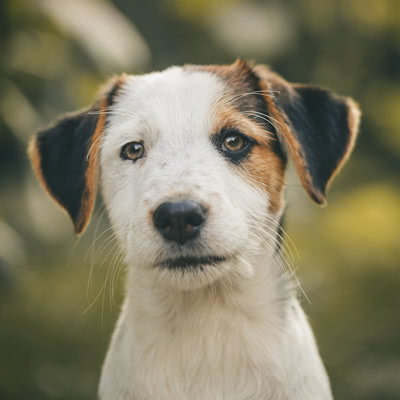
\includegraphics[width=0.5\textwidth]{figures/front_page/dog.jpg}\\
    %     \includegraphics[width=0.5\textwidth]{figures/front_page/molly.jpeg}\\
    %     \end{figure}
    %     \thispagestyle{empty}
    % \end{titlepage}

    \newpage
    \label{sec:eyyy}


    \section{Introduction}\label{sec:introduction}

Cell membranes are the foundation of the origin of life, but also linked to the dynamics of virus al infections and genetic mutations since it controls what substances that can exit or enter the cell \cite{ hurley2010membrane}. In fact, a good
understanding of the cell membrane is important of engineering proteins to manipulate various intracellular processes in living systems \cite{rojas1998genetic}.

One of the primary components of the cell membranes are lipids which serve many different functions. A key function is that it is consisting of a bilayer of lipids which controls the structural rigidity and the fluidity of the membrane. Thus, elastic
bending forces, temperature and diffusion is essential on how a cell membrane will evolve \cite{udo97,neidleman87}.


\subsection{Elastic bending energy on evolving surfaces}%
\label{sub:willmore_flow}

Assuming that the system is a single-phase system, i.e., the lipids are uniformly distributed, can the elastic bending energy be modelled using the Canham-Helrich energy functional \cite{helfrich1973elastic, wang08, udo97}. Let us denote $b_{b},
b_{k}$ and $H_{0}$ as parameters based on physical models, then can the energy functional be denoted as,
\begin{equation}
\label{eq:CH}
\mathcal{E} _{CH}\left( \Gamma\left( t \right)   \right) =   \int_{\Gamma  }^{}  b_{b} \left( H- H_{0} \right) ^{2} + b_{k} K
.\end{equation}
Here is $H =  \kappa_1 + \kappa_2 $ denoted as the mean curvature and $K = \kappa_1 \kappa_2$ as the gaussian curvature with respectively and $\kappa_1$ and $\kappa_2$ as principal curvatures. $\Gamma \left( t
\right) = \Gamma  $ is here an evolving surface in $\mathbb{R} ^3$, for more info see section \ref{sec:background}.  Using the Gauss-Bonnet theorem can it be shown that the problem above is equivalent to the so-called Willmore energy
functional \cite{montiel2009curves, willmore1996riemannian},

\begin{equation}
\label{eq:WE}
\mathcal{E} _{W} \left( \Gamma\left( t \right)   \right) = \int_{\Gamma  }^{} \frac{1}{2} H ^2
.\end{equation}

This is a well known problem in the mathematical community \cite{ topping2000towards, marques2014willmore,link2013gradient,kuwert2012willmore}. In fact, it is a mathematical tool used to study the geometry of surfaces because it can be used to study
the diffeomorphism from a initial surface to a minimal energy configuration, which are surfaces with the least possible area for a given boundary. This is important in many areas of mathematics, including differential geometry, topology and mathematical physics \cite{koerber2021area,jakob2022singularities, rupp21}.

It has been established many numerical methods for for shape optimization problems \cite{sokolowski1992introduction,ito2008variational}, evolving surface partial differential equations (PDE) \cite{dziuk2013finite, dziuk2007finite,
binz2022convergent, barrett2007parametric, barrett2007variational, kovacs2019convergent, lehrenfeld2018stabilized} and specific
algorithms for the Willmore energy problem \eqref{eq:WE} \cite{palmurella2022parametric, dziuk2008computational, bonito2010parametric,  kovacs2021convergent, hu2022evolving}.

\subsection{Two-phase separation modelling on predefined evolving surfaces }%
\label{sub:two_phase_seperation_modelling_on_surfaces_}

It also turns out that the lipids often accumulate into so-called lipid rafts which serves as a rigid platform for proteins with special properties such as intracellular trafficking of lipids and lipid-anchored proteins \cite{ miller2020divide}. Modelling of
lipid rafts formation can be modelled as a two-phase separation problem based on minimization of the Ginzburg-Landau energy functional \cite{yushutin19},
\begin{equation}
\label{eq:GL}
\mathcal{E}_{GL}  \left( c   \right) = \int_{\Gamma\left(t  \right)   }^{}\Psi \left( c \right) + \frac{\gamma}{2} \left\lvert \nabla c \right\rvert^{2} ,
\end{equation}
which describes the chemical energy for a concentration $c: \Gamma\left( t \right)  \times \left[ 0,T \right] \mapsto  \left[ 0,1 \right]  $. Here is $ \Psi \left( c \right): \mathbb{R} \mapsto \mathbb{R} $ denoted as a nonlinear scalar chemical potential function. Keep in mind that unlike
the Willmore energy functional \eqref{eq:WE}, where the $\Gamma\left( t \right)  $ is determined by the elastic properties, should the energy functional \eqref{eq:GL} be interpreted as a chemical diffusion problem a predefined evolving domain $\Gamma \left( t \right) $.
Usually is this problem solved by deriving equivalent variants of partial differential equations (PDE) such as Allen-Cahn equation (or Cahn-Hilliard equation if the total concentration is globally conserved) on evolving domains. For further details,
see \cite{yushutin19,
udo97, ratz16,Gera2017, caetano21, elliott2015evolving}.

\subsection{Multiphysics problems on evolving surfaces}%

Ultimately will the cell membrane consists of interaction several kinds of physics (temperature, elasticity, chemical diffusion, internal fluid pressure etc.) \cite{udo97}. Hence, being able to model several processes may give unforeseen results.

An interesting example is to couple the energy functionals \eqref{eq:GL}  and \eqref{eq:CH}, since the lipid-rafts formation is said to change the elasticity properties of the membrane, may be a good model for how cell membranes evolve to specific shapes or execute cell division. One way
to couple the energy functionals is to let the parameters $b_{b}, b_{k}$ and $ H_{0} $ be some function of the time dependent concentration $c$, i.e.,
\[
    \begin{split}
        \mathcal{E}_{CHGL} \left( \Gamma\left( t \right) ,c\left( t \right)    \right) =  & \int_{\Gamma  }^{}  b_{b}\left( c \right)  \left( H- H_{0}\left( c \right)  \right) ^{2}  \\
        & + \int_{\Gamma   }^{} b_{k}\left( c \right)  K \\
        &+ \int_{\Gamma   }^{}\Psi \left( c \right) + \frac{\gamma}{2} \left\lvert \nabla c \right\rvert^{2} ,
    \end{split}
\]
For more information, see \cite{elliott2010surface}.

Recently have some authors also coupled diffusion processes and the so-called mean curvature energy, see \cite{burger2021interaction, elliott2022numerical}. It is well known that lipids travels
along the cell membrane in a fluidic manner, hence, it is also of interest to couple the Ginzburg-Landau energy functional \eqref{eq:GL} (or more specifically the Cahn-Hilliard equation) with the Navier-Stokes equation. Some methods has been proposed
methods for solving the problem on surfaces
and evolving surfaces, but it remains a field of active research \cite{olshanskii2022comparison}. As far as a author knows, coupling the Canham-Helrich energy functional \eqref{eq:CH}, Ginzburg-Landau energy functional \eqref{eq:GL}  and Navier-Stokes equation remains a open problem.

Some physical processes may require constant area and volume. This can simply be added by introducing respectively area and volume functionals, see \cite[Definition 2.5]{muller2013volume}.

Until now have all the models assumed that the membrane has no difference in internal and external pressure. As a matter of fact, osmotic pressure can be introduced by adding a energy functional using the van't Hoff formula. Let $V_{p}$ be the volume
of a closed evolving surface $\Gamma \left( t \right) $, we can then model the difference of internal and external pressure as,
\[
\Delta P \left( V_{p} \right) = P_{in} - P_{out} = iRT\left( \frac{n}{V_{p}} - \overline{c}  \right),
\]
where $i, R, T, \overline{c} $ and $n$ are the van't Hoff index, ideal gass constant, temperature , ambient molar concentration and molar amount of the enclosed solute. Then the energy
functional have the form,
\[
\mathcal{E} _{p}\left( \Gamma    \right)  = \int_{\Gamma   }^{   } \Delta P\left( V_{p} \right) ,
\]
For more information, see \cite{zhu2022mem3dg}.


\subsection{Outline of this report}%
\label{sub:outline_of_this_report}

The long-term goal would be to solve the multi-physics problems above. However, many of the problems above is fairly complicated to solve numerically and requires sophisticated techniques. Hence, in this report we focus on the latest research withing
the numerical methods of finding the minima of the energy functional \eqref{eq:WE}. However, we will first establish notation by including a section for definitions and important results from differential geometry and shape derivatives. We will then derive the
underlying dynamics system of evolutionary system dynamics using the gradient flow technique inspired by shape optimization methods based on the work done in \cite{ dougan2012first}. Lastly, we will establish the numerical methods of the system
dynamics by applying recent methods using an evolutionary surface finite element method (FEM) \cite{kovacs2021convergent, hu2022evolving}.



    \input{biharmonic-equation}
    \newpage
\section{Continuous Interior Penalty Method}%
\label{sec:continious_interior_penalty_method}


\subsection{Introduction}%
\label{sub:introduction}

To solve \eqref{eq:bi_problem} numerically do we want to introduce the continuous interior penalty method (CIP), which is a discontinuous Galerkin
method (DG) using $C^{0}$ finite elements. There is several reasons why we want to apply nonconformal $C^{0}$ instead of the often used conformal $C^{1}$ finite elements for fourth order problems.

However, it is known that $ H^{2}$ conforming methods requires global $C^{1}$ continuity \cite{ye19}, and creates difficulties creating elements which conserves this property. Some examples is the Argyris element, but it has been shown to be fairly
complicated because you have to construct 21 degrees of freedom for triangle elements \cite{ nair21, brenner07math}. However, some sources tend to say that this method outperforms traditional $C^{0}$ methods \cite{kirby18}, but it still seems to be rarely applied.
Nevertheless, it has also been shown DG methods that is conform and has no penalty terms that does converge \cite{ye19}. Hence, makes the method simpler since it does not involve tuning of penalty parameters, thus might be promising. None of these conform methods mentioned has shown to retain the same properties in 3D.

For the CIP case is $C^0$ finite elements much simpler than obtaining $C^{1}$ finite elements. Also, compared to other similar methods such as the mixed finite element method, CIP does in fact preserve the symmetric positive definiteness, which means
the stability analysis is more straight forward. Finally and most importantly, according to \cite{brenner2012quadratic} can naive use mixed methods of splitting the boundary conditions of
the problem \eqref{eq:bi_problem} produce wrong solutions if $\Omega $ is non convex.

\subsection{Computational Domains}%
\label{sub:computational_domain}

Let $\mathcal{T}  = \left\{ T \right\} $ be a triangulation of $\Omega \subset   \mathbb{R} ^2 $ consisting of triangles $T$. We may also define the set of all facets $\mathcal{F}_{h}$, where every facet is denoted by $F \in \mathcal{F} _{h}$. However, we will distinguish between the
set of external facets $\mathcal{F}^{ext} _{h}$, which is all facets along $\partial \Omega $, and the interior facets $\mathcal{F} ^{int}_{h}$. Let the facets be denotes as $F \in \mathcal{F } _{h}$, then the normal vector $n$ is across the facets from
$T^{+}$ to $T^{-}$, illustrated in figure \ref{fig:normal}.

\begin{figure}[!h]
\centering
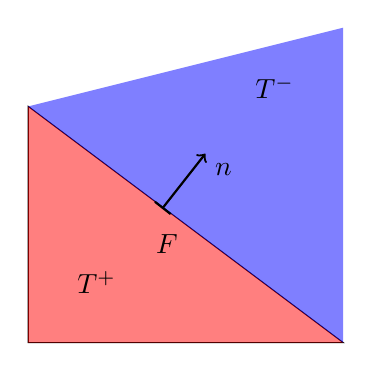
\begin{tikzpicture}[scale=1]
\coordinate (A) at (0,0);
\coordinate (C) at (0,3);
\coordinate (B) at (4,0);
\coordinate (D) at (4,4);
\coordinate (Tm) at (3.5,3.5);
\coordinate (Tp) at (0.5, 0.5);
\coordinate (e) at (1.5, 1.5);
\coordinate (start) at (1.7, 1.7);
\coordinate (end) at (2.25, 2.4);

\draw (A) -- (B) -- (C) -- cycle;
\fill[red, opacity=0.5] (A) -- (B) -- (C);
\fill[blue, opacity=0.5] (B) -- (C) -- (D);
\node[below left] at (Tm) {$T^{-} $ };
\node[above right] at (Tp) {$T^{+}$ };
\node[below right] at (e) {$F$ };

\draw [|->, thick] (start) -- (end);
% \node[above right] at (A) {A };
% \node[below right] at (B) {B};
% \node[above right] at (C) {C };
% \node[below right] at (D) {D};
\node[below right] at (end) {$n$};
\end{tikzpicture}
\caption{Facet $F \in \mathcal{F}_h $ shared by the triangles $T^{+}, T^{-} \in \mathcal{T}_{h} $ and the normal unit vector $n$.  }
    \label{fig:normal}
\end{figure}

A parameter which is useful is the maximum diameter $h$ of the set of triangles $\left\{ T \right\} $, which we to be defined such that,

\begin{equation}
\begin{split}
    h _{T} & = diam\left( T \right)   = \max_{x_1, x_{2} \in T} dist(x_{1}, x_{2}),  \\
    h_{min} & = \min_{T \in \mathcal{T} } h_{T}, \\
    h_{max} &= \max_{T \in \mathcal{T} }  h_{T} := h,
\end{split}
.\end{equation}




where the $diam( T )$ is the largest facet for a triangle $T$. We will also assume mesh conform i.e., if $T_{1} \neq T_{2 }$  and $T \cap T_{2} \neq \emptyset  $ , then they share either a vertex or a facet.

Let the chunkiness parameter $c_{T} := h_{T}/r_{T}$, where $r_{T}$  is the largest ball that be inscribed inside the element $T$. We can then assume that the mesh is shape regular, i.e., that $c_{T}\le  c$ independent of $T$  and $h$. We may also assuming that
the mesh is quasi-uniform only if it holds that the mesh is shape regular and $h_{max} \le  c h_{min}$.




\subsection{Constructing Continuous Interior Penalty Method}%
\label{sub:constructing_continious_interior_penalty_method}

 Let us assume that $u,v \in
H^{4}\left( T  \right) $. Using that the weak form identity \eqref{eq:weak_form_identity} also holds for a triangle $T$ can we write
\begin{equation}
\label{eq:bi_basic_dg}
\left( \Delta  ^{2} u,v \right) _{T} =  \left( D^2u,D^2v \right) _{T } - \left(\partial _{nt} u, \partial _{t}v
\right)_{\partial T} - \left(\partial _{nn} u, \partial _{n}v \right)_{\partial T} + \left(\partial _{n} \Delta  u,v
\right)_{\partial T}
.\end{equation}
For global continuity, let  $v \in V =  \left\{ v \in H^{1}\left( \Omega  \right): v_{T} \in  H^{4}\left( T \right), \ \forall T \in
\mathcal{T}_{h}    \right\} $ and $u \in  H^{4}\left( \Omega  \right) $ such that,

\begin{equation}
\label{eq:bi_basic_dg2}
\left( \Delta  ^{2} u,v \right) _{\Omega } = \sum_{T \in  \mathcal{T} _{h}}^{}  \left( D^2u,D^2v \right) _{T } - \left(\partial _{nt} u, \partial _{t}v
\right)_{\partial T} - \left(\partial _{nn} u, \partial _{n}v \right)_{\partial T} + \left(\partial _{n} \Delta  u,v
\right)_{\partial T}.
\end{equation}
However, this expression can be written to distinguish integrating over triangles $\mathcal{T} _{h}$ , integrating over exterior facets $\mathcal{F} _{h}^{ext}$ and then integrate interior facets $\mathcal{F} _{h}^{int}$.

\begin{equation}
\label{eq:bi_basic_dg_full_1}
\begin{split}
\left( \Delta  ^{2} u, v \right) _{\Omega } =& \sum_{T \in  \mathcal{T} _{h}}^{} \left( D^2u, D^2v \right)_{T}    \\
& + \sum_{F \in \mathcal{F}_{h}^{ext}}  \left(\partial _{n} \Delta u, v  \right) _{F} - \left(\partial _{nt} u, \partial _{t} v \right) _{F}-
\left( \partial _{nn} u, \partial _{n} v \right)_{F}  \\
& + \sum_{F \in \mathcal{F}_{h}  ^{int}}^{} \left(\partial _{nn} u , \jump{ \partial _{n} v }
\right)_{F} \\
& = \sum_{T \in  \mathcal{T} _{h}}^{} \left( D^2u, D^2v \right)_{T} + \sum_{F \in
\mathcal{F} ^{ext}_{h}}^{} \left(g, v  \right) _{F}
  + \sum_{F \in \mathcal{F}  ^{int}}^{} \left( \partial _{nn} u , \jump{ \partial_{n} v } \right)_{F}
\end{split}
\end{equation}
Keep in mind that any jump over a interior facet $F \subset \mathcal{F} _{h}^{int}   $, visualized in figure \ref{fig:normal}, is defined as $\jump{ a } =    a^{+} - a^{-} $
and likewise for the mean, $\mean{ a  } = \frac{1}{2}(   a^{+}
+ a^{-})$.    The equivalence of \eqref{eq:bi_basic_dg2} and \eqref{eq:bi_basic_dg_full_1} comes from the following argumentation.

\begin{equation*}
    \begin{split}
 \left( \Delta  ^{2} u,v \right) _{\Omega } & =\sum_{T\in \mathcal{T} _{h}}^{} \left( D^2u,D^2v \right) _{T } - \left(\partial _{nt} u, \partial _{t}v
\right)_{\partial T} - \left(\partial _{nn} u, \partial _{n}v \right)_{\partial T} + \left(\partial _{n} \Delta  u,v
\right)_{\partial T} \\
&= \sum_{T\in \mathcal{T} _{h}}^{} \left( D^2u,D^2v \right) _{T } \\
&  \quad + \sum_{F \in \mathcal{F}_{h}^{ext} }^{} \underbrace{\left( \partial _{n} \Delta  u, v  \right)_{F}}_{= \left( g,v \right)_{F} }  -  \left(
\partial _{nt} u, \partial _{t} v \right) _{F}  - \underbrace{\left( \partial _{nn} u, \partial _{n} v \right)_{F}}_{ = 0}    \\
& \quad  + \sum_{F \in \mathcal{F} _{h}^{int}}^{} \underbrace{\left( \left(\partial _{n^{+}} \Delta  u^{+}
        ,v^{+}\right)_{F}
+ \left(\partial _{n^{-}} \Delta  u^{+} ,v^{-}\right)_{F}  \right)}_{(I)} \\
 & \quad \quad \quad  \quad +
\underbrace{\left( \left(\partial _{n^{+}t} u^{+}, \partial_{t} v^{+} \right)_{F} +  \left(\partial _{n^{-}t} u^{-},
        \partial_{t} v^{-}
\right)_{F}  \right) }_{(II)} \\
 & \quad \quad \quad  \quad  +
\underbrace{\left( \left(\partial _{n^{+}n^{+}} u^{+}, v^{+} \right) _{F} + \left(\partial _{n^{-}n^{-}} u^{-}, v^{-}
\right) _{F} \right) }_{(III)}
    \end{split}
.\end{equation*}

Where integration over all interior facets $ \forall F \in \mathcal{F}_{h}^{int}$ is computed in this way.
\begin{equation*}
    \begin{split}
        (I) &  =    \left(\partial _{n^{+}} \Delta  u^{+} ,v^{+}\right)_{F} +
        \left(\partial _{n^{-}} \Delta  u^{+} ,v^{-}\right)_{F}  \\
        & =   \int_{F}^{}
        \jump{ \partial _{n} \Delta  u \cdot v } =
         \int_{F}^{}
         \mean{ \partial _{n} \Delta  u } \underbrace{\jump{ v }}_{= 0}    + \underbrace{\jump{ \partial _{n} \Delta  u
         }}_{= 0}    \mean{ v } = 0 \\
        (II) &  =     \left(\partial _{n^{+}t} u^{+}, \partial_{t} v^{+}
        \right)_{F} +  \left(\partial _{n^{-}t} u^{-}, \partial_{t} v^{-}
\right)_{F}   \\
&  =   \int_{F}^{}
        \jump{ \partial _{nt} u \cdot  \partial_{t} v } =
         \int_{F}^{}
         \mean{ \partial _{nt} u    } \underbrace{\jump{ \partial_{t} v }  }_{= 0}    + \underbrace{\jump{ \partial
                 _{nt}  u
         }}_{= 0}    \mean{ \partial _{t}v }  = 0\\
        (III) &  =     \left(\partial _{n^{+}n^{+}} u^{+}, \partial_{n^{+}} v^{+} \right)_{F} +  \left(\partial _{n^{-}n^{-}} u^{-}, \partial_{n^{-}} v^{-} \right)_{F}    =    \int_{F}^{} \jump{ \partial _{nn} u \cdot  \partial_{n} v }  \\
        & = \int_{F}^{}
        \mean{ \partial _{nn} u    } \underbrace{\jump{ \partial_{n} v }  }_{\neq 0}    + \underbrace{\jump{ \partial
                 _{nn}  u
         }}_{= 0}    \mean{ \partial _{n}v }   =  \left( \partial _{nn} u, \jump{ \partial_{n} v } \right)_{F}   \end{split}
.\end{equation*}
Observe that the cancellations in the term $(I)$ appears of the continuity of $v\in V $ and $u\in H^{4}\left( \Omega  \right) $ which makes the jumps zero. For the second term $(II)$ does the terms become zero cancelled because the tangential
derivative at the facet has no jump. However, The third term $(III)$  is fairly interesting since the discontinuity in
normal vector for $v \in V$ is a jump, while the second term is still continuous. It can also be raised that $\mean{
\partial _{nn} u } = \partial _{nn} u  $ holds by the continuity of $H^{4}\left( \Omega  \right) $. Hence,
\eqref{eq:bi_basic_dg2} and \eqref{eq:bi_basic_dg_full_1} is equivalent.

\subsection{Formulation of the Continious Interior Penalty Method}%
\label{sub:formulation_of_continious_interior_penalty_method}


We can finally start defining the fully discrete formulation. Let the basis be a $\mathcal{P}_{2} $ Lagrange finite element space so,
\[
V_{h} = \left\{ v \in C^{0}\left( \Omega  \right): v_{T} = v | _{T} \in \mathcal{P} _{2}\left( T \right), \forall T \in
\mathcal{T}_{h}    \right\}
\]
and
\[
V_{h}^{*} = \begin{cases}
    V_{h} & \text{ if } \alpha  > 0 \\
    \left\{ v \in V_{h}: \int_{\Omega }^{} v dx   = 0   \right\} &  \text{ if } \alpha   = 0
\end{cases}
\]
Now, if we choose $u \in V_{h}$, then we must take account that the jump is discrete.
 Finally, the CIP formulation can be stated as follows.
The discretized numerical problem is to solve $w_{h} \in V_{h}^{*}$ such that
\begin{equation}
\label{eq:CP_A_F}
\mathcal{A}\left( w_{h}, v_{h} \right)   = F\left( v_{h} \right), \quad \forall v_{h} \in V_{h}^{*}  .
\end{equation}
where
\begin{equation}
\label{eq:CP_A_h_1}
\begin{split}
\mathcal{A} \left( w_{h}, v_{h} \right)   =&
  \quad  \left( \alpha  w_{h}, v_{h} \right) _{\Omega }\\
&  + \sum_{T \in \mathcal{T} _{h}}^{} \left( D^2 w_{h}, D^2v_{h} \right) _{T} \\
 & +
  \sum_{F \in \mathcal{F}_{h}^{int} }^{}
  \left( \mean{  \partial _{n n} w_{h} }, \jump{ \partial _{n }v_{h}} \right)_{F}  +
 \left( \mean{ \partial _{n n} v_{h} }, \jump{ \partial _{n}w }      \right)_{F} \\
& \quad \quad \quad \quad  + \frac{\gamma}{h}  \left( \jump{ \partial _{n} w_{h}}, \jump{ \partial _{n} v_{h}   }   \right)_{F}
\end{split}
\end{equation}
and
\begin{equation}
\label{eq:CP_F_h}
F\left( v_{h} \right)  = \left( f, v_{h} \right) _{\Omega } +  \sum_ {F \in \mathcal{F}_{h} ^{ext}}^{} - \left(g, v_{h}  \right) _{F}.
\end{equation}
Notice that the regulation term determined by respectively a global tuning parameter $\gamma >0 $. Another key component to the formulation
in \eqref{eq:CP_A_h_1} after introduction of $ w_{h}, v_{h} \in V^{*}_{h}$  is that we expanded $\left( \partial _{nn}w, \jump{ \partial _{n} v }  \right)_{F} \to \left( \mean{ \partial _{nn}w_{h} }  , \jump{ \partial _{n} v_{h} }  \right)_{F} $ since we can longer not guarantee a
continuous jump. For symmetric purposes we also added $ \left( \mean{ \partial _{nn} v_{h}}  , \jump{ \partial _{n} w_{h} }  \right)_{F} $. For convenience will we introduce the compact notation of \eqref{eq:CP_A_h_1},

\begin{equation}
\label{eq:CP_A_h}
\begin{split}
\mathcal{A} \left( w_{h}, v_{h} \right)   =&
  \quad  \left( \alpha  w_{h}, v_{h} \right) _{\Omega }\\
&  +  \left( D^2 w_{h}, D^2v_{h} \right) _{\mathcal{T} _{h}} \\
 & +
  \left( \mean{  \partial _{n n} w_{h} }, \jump{ \partial _{n }v_{h}} \right)_{\mathcal{F}_{h}}  +
 \left( \mean{ \partial _{n n} v_{h} }, \jump{ \partial _{n}w }      \right)_{\mathcal{F}_{h}}
 \\
 & + \frac{\gamma }{h}  \left( \jump{ \partial _{n} w_{h}}, \jump{ \partial _{n} v_{h}   }   \right)_{\mathcal{F}_{h}} \\
\end{split}
.
\end{equation}

\subsection{ Stability Results}%
\label{sub:error_and_stability_analysis_of_c0ip}

To guarantee convergence and stability we may want to check coercivity and boundedness of the method.

First of all, let us now establish some important inequalities.
\[
\begin{split}
    \textbf{Cauchy-Schwarz inequality: } & \| ab \|_{  }^{  }  \le \| a \|_{  }^{  } \| b \|_{  }^{  }   \\
    \textbf{Inverse inequality: } & \frac{1}{h}\| \partial _{nn}  v_{h} \|_{\mathcal{F}_{h}   }^{2  }  \le C_{j} \| D ^2 v_{h} \|_{ \mathcal{T} _{h} }^{ 2 }   \\
    \textbf{Youngs epsilon inequality: } & 2ab =   2\sqrt{\varepsilon }a\cdot    \frac{b}{\sqrt{\varepsilon } } \le \varepsilon a^2+ b^2 \frac{1}{\varepsilon }
\end{split}
\]

Let the energy norm be on the form,
\begin{equation}
\label{eq:A_energy_norm}
    \begin{split}
\| v_{h} \|_{ h }^{2  } & = \| v_{h} \|_{ a_{h} }^{ 2 } =  \| v_{h} \|_{ \Omega  }^{2  }  +  \| D ^2 v_{h} \|_{ \mathcal{T} _{h}  }^{ 2 }  + \|  h^{-\frac{1}{2}} \jump{ \partial _{n} v_{h}    }\|_{  \mathcal{F} _{h} }^{2  }, \\
\| v \|_{ h }^{ 2 }  &= \| v \|_{ a_{h},* }^{ 2 } = \| v \|_{ a_{h} }^{ 2 }  + \| h^{\frac{1}{2}} \left\{ \partial _{nn } v\right\}  \|_{ \mathcal{F}_{h}   }^{  2}, \quad  v\in V \oplus V_{h}.
    \end{split}
\end{equation}
The method is said to be coercive if $\mathcal{A} _{h}\left( v_{h}, v_{h} \right) \ge  C \| v_{h} \|_{ a_{h} }^{  } $. Similarly, it is bounded if $ \mathcal{A} _{h} \left( v_{h}, u_{h} \right) \le  C \| u_{h} \|_{  a_{h}}^{ 2 }  \| v_{h} \|_{ a_{h}
}^{ 2 } $ and then, according to Lax Milgram the problem is said to be well posed.

\subsubsection{Coercivity}%
\label{ssub:coercitivity}


Suppose we have the CIP problem described in \eqref{eq:CP_A_F}. Then is the coercivity be computed such that,
\[
    \begin{split}
\mathcal{A} \left( v_{h}, v_{h} \right)  =& \quad  \alpha \|  v_{h}  v_{h} \|_{ \Omega  }^{  } +  \| D^2v_{h} \|_{ \mathcal{T} _{h} }^{2  }   \\
& \quad + 2 \left(  \mean{ \partial _{nn} v_{h} }    ,  \jump{ \partial _{n}v_{h} }     \right) _{\mathcal{F} _{h}} +  \frac{\gamma}{h} \|  \jump{ \partial _{n} v_{h} }
  \|_{ \mathcal{F} _{h} }^{ 2 } \\
\quad \textit{Cauchy-Schwarz inequality} \quad
 \ge& \quad  \alpha \| v_{h}  \|_{\Omega   }^{  } \| v_{h} \|_{\Omega   }^{  } +   \| D ^2 v_{h} \|_{ \mathcal{T} _{h} }^{2  } \\
& \quad -2 \| h^{\frac{1}{2}} \mean{ \partial _{nn}v_{h} }    \|_{  \mathcal{F} _{h}}^{  } \| h^{-\frac{1}{2}} \jump{ \partial _{n}v_{h} }    \|_{  \mathcal{F} _{h}}^{  } + \gamma \| h^{-\frac{1}{2}}  \jump{ \partial _{n}v_{h} }   \|_{ \mathcal{F} _{h}  }^{ 2 } \\
\quad \textit{Inverse inequality} \quad
   \ge & \quad  \alpha \| v_{h}  \|_{\Omega   }^{  } \| v_{h} \|_{\Omega   }^{  } + \| D ^2 v_{h}  \|_{ \mathcal{T} _{h}  }^{ 2  }  \\
 &  \quad - 2 C^{\frac{1}{2}}_{j} \|   D ^2 v_{h}    \|_{ \mathcal{T} _{h}  }^{  } \| h^{-\frac{1}{2}} \jump{ \partial _{n} v_{h} }   \|_{ \mathcal{F} _{h} }^{  }  + \gamma \| h^{ -\frac{1}{2}} \jump{
 \partial _{n } v_{h}}   \|_{ \mathcal{F}_{h}}^{2}  \\
\quad \textit{ Youngs epsilon inequality} \quad
    \ge  &  \quad  \alpha \| v_{h}  \|_{\Omega   }^{  } \| v_{h} \|_{\Omega   }^{  } +  \| D ^2 v_{h} \|_{ \mathcal{T}_{h}  }^{2  } - \varepsilon C_{j} \| D ^2 v_{h} \|_{ \mathcal{T} _{h} }^{2  } \\
  & \quad  - \frac{1}{\varepsilon } \| h^{\frac{1}{2}} \jump{ \partial _{n} v_{h} }   \|_{ \mathcal{F} _{h} }^{2  }  + \gamma \|
  h^{-\frac{1}{2}} \jump{ \partial _{n} v_{h}}   \|_{ \mathcal{F} _{h} }^{2  }  \\
   =&  \quad  \alpha \| v_{h}  \|_{\Omega   }^{  } \| v_{h} \|_{\Omega   }^{  } +\left( 1 - \varepsilon C_{j} \right) \| D ^2 v_{h} \|_{\mathcal{T} _{h}  }^{ 2 }  \\
  & \quad + \left( \gamma  - \frac{1}{\varepsilon } \right) \| h^{-\frac{1}{2}} \jump{ \partial _{n} v_{h} }   \|_{ \mathcal{T} _{h} }^{ 2 } \\
  (\varepsilon  = \frac{1}{2 C_{j} })  \implies  \quad \quad =& \quad  \alpha \| v_{h}  \|_{\Omega   }^{  } \| v_{h} \|_{\Omega   }^{  } +\frac{1}{2} \| D ^2 v_{h} \|_{ \mathcal{T} _{h} }^{ 2 }  + \underbrace{\left( \gamma -2 C_{j} \right)}_{ \ge  \frac{1}{2}}  \| h^{\frac{1}{2}} \jump{ \partial _{n} v_{h} }   \|_{
  \mathcal{F} _{h} }^{2  } \\
   \ge & \quad  C \| v_{h} \|_{ a_{h} }^{  2}
    \end{split}
\]
This holds if $C=\min\left\{  \alpha , 1 /2\right\}$.
Observe that for the first inequality is the standard \textbf{Cauchy-Schwarz inequality} such that $$\left( \mean{ \partial_{nn} v_{h} }  , \jump{ \partial _{n} v_{h} }   \right) _{\mathcal{F} _{h}} \ge - \| h^{-\frac{1}{2}} \mean{ \partial _{nn}
v_{h} }    \|_{\mathcal{F}_{h}   }^{  } \| \mean{ \partial _{n}v_{h} }   \|_{ \mathcal{F}_{h}   }^{  } .  $$ On the second inequality the \textbf{Inverse inequality} was applied,
\[
- \| h^{\frac{1}{2}} \mean{ \partial _{nn}v }   \|_{ \mathcal{F} _{h}  }^{  }\ge - C_{j}^{\frac{1}{2}} \| D ^2 v_{h} \|_{ \mathcal{T} _{h} }^{  }
\]
The next step is then to use the \textbf{Youngs epsilon inequality} to separate the facets and triangulation norms, \[
 - 2 C^{\frac{1}{2}}_{j} \|  D ^2 v_{h}    \|_{ \mathcal{T} _{h}  }^{  } \| h^{\frac{1}{2}} \jump{ \partial _{n} v_{h} }   \|_{ \mathcal{F} _{h} }^{  } \ge- \varepsilon C_{j} \| D ^2 v_{h} \|_{ \mathcal{T} _{h} }^{2  } -
 \frac{1}{\varepsilon } \| h^{\frac{1}{2}} \jump{ \partial _{n} v_{h} }   \|_{ \mathcal{F} _{h} }^{2  }
.\]
The last step was to choose a $\varepsilon $ and $\gamma $ as some positive constant so that the second term is restricted to be multiplied with something bigger than $\frac{1}{2}$. Thus, the term fulfils coercivity of the \eqref{eq:A_energy_norm}.
Hence, the CIP method is coercive.

\subsubsection{Boundedness}%
\label{ssub:bounded}
We want the CIP method to be bounded.


\begin{equation*}
    \begin{split}
\mathcal{A} \left( w_{h}, v_{h} \right)   =& \quad \left( \alpha w_{h}, v_{h} \right) _{\Omega } +
    \left( D ^2 w_{h}, D ^2v_{h} \right) _{\mathcal{T} _{h}}
   \\
    &\quad  +
  \left( \mean{  \partial _{n n} w_{h} }, \jump{ \partial _{n }v_{h}} \right)_{\mathcal{F}_{h}}  +
 \left( \mean{ \partial _{n n} v_{h} }, \jump{ \partial _{n}w }      \right)_{\mathcal{F}_{h}} \\
 & \quad + \frac{\gamma }{h}  \left( \jump{ \partial _{n} w_{h}}, \jump{ \partial _{n} v_{h}   }   \right)_{\mathcal{F}_{h}} \\
\quad \textit{Cauchy-Schwarz inequality }\quad  \le& \quad  \alpha  \|  w_{h} \|_{\Omega   }^{  } \| v_{h} \|_{ \Omega  }^{  }     +
\| D ^2w_{h} \|_{\mathcal{T} _{h}   }^{  }  \| D ^2v_{h} \|_{\mathcal{T} _{h}   }^{  } \\
& \quad  + \| h^{\frac{1}{2}}\mean{ \partial _{nn} w_{h} } \|_{ \mathcal{F}_{h}  }^{  } \| h^{-\frac{1}{2}}\jump{ \partial _{n} v_{h} } \|_{ \mathcal{F}_{h}  }^{  }    \\
& \quad  + \| h^{\frac{1}{2}}\mean{ \partial _{nn} v_{h} }
\|_{ \mathcal{F}_{h}  }^{  } \| h^{-\frac{1}{2}}\jump{ \partial _{n} w_{h} } \|_{ \mathcal{F}_{h}  }^{  }  \\
& \quad + \gamma \| h^{-1} \jump{ \partial _{n} v_{h}}   \|_{ \mathcal{F} _{h} }^{  }   \|  \jump{ \partial _{n} w_{h}}   \|_{ \mathcal{F} _{h} }^{  } \\
\quad \textit{Inverse inequality }\quad  \le & \quad   \alpha  \|  w_{h} \|_{\Omega   }^{  } \| v_{h} \|_{ \Omega  }^{  }  +
\| D ^2w_{h} \|_{\mathcal{T} _{h}   }^{  }  \| D ^2v_{h} \|_{\mathcal{T} _{h}   }^{  } \\
& \quad + C_{j}^{\frac{1}{2}} \| D ^2 w_{h} \|_{\mathcal{T} _{h}  }^{  }  \| h^{-\frac{1}{2}}\jump{ \partial _{n} v_{h} } \|_{ \mathcal{F}_{h}  }^{  }
 \\
& \quad +  C_{j}^{\frac{1}{2}} \| D ^2 w_{h} \|_{\mathcal{T} _{h}  }^{  }
 \| h^{-\frac{1}{2}}\jump{ \partial _{n} w_{h} } \|_{ \mathcal{F}_{h}  }^{  }\\
 & \quad  + \gamma \| h^{-1} \jump{ \partial _{n} v_{h}}   \|_{ \mathcal{F} _{h} }^{  }   \|  \jump{ \partial _{n} w_{h}}   \|_{ \mathcal{F} _{h} }^{  } \\
\textit{ Using \eqref{eq:bounded_ineq}}  \quad  \le & \quad \alpha  \|  w_{h} \|_{a_{h}   }^{  } \| v_{h} \|_{ a_{h}   }^{  } + \| w_{h} \|_{ a_{h} }^{  } \| v_{h} \|_{ a_{h} }^{  }  + 2C_{j}^{\frac{1}{2}} \| w_{h} \|_{ a_{h} }^{  } \| v_{h} \|_{
a_{h} }^{  }  \\
 & \quad + \gamma \| v_{h} \|_{ a_{h} }^{  } \| w_{h} \|_{ a_{h} }^{  } \\
 \le& \quad   \left( \alpha + 1 + 2C_{j}^{\frac{1}{2}} + \gamma  \right)  \| v_{h} \|_{a_{h}  }^{  }  \| w_{h} \|_{ a_{h} }^{  }  \le  K  \| v_{h} \|_{a_{h}  }^{  }  \| w_{h} \|_{ a_{h} }^{  }
\end{split}
\end{equation*}

Thus, the CIP method is shown to be bounded.
Again, the first step was to apply the \textbf{Cauchy-Schwarz inequality} for every term. On the second inequality the \textbf{Inverse inequality} was applied so that
\[
\| h^{\frac{1}{2}} \mean{ \partial _{nn}v_{h} }   \|_{ \mathcal{F} _{h}  }^{  }\le   C_{j}^{\frac{1}{2}} \| D ^2 v_{h} \|_{ \mathcal{T} _{h} }^{  } \quad \text{and} \quad   \| h^{\frac{1}{2}} \mean{ \partial _{nn}w_{h} }   \|_{ \mathcal{F} _{h}
}^{  }\le   C_{j}^{\frac{1}{2}} \| D ^2 w_{h} \|_{ \mathcal{T} _{h} }^{  }.
\]
The second step can we luckily observe that all terms invidually is less than the norm, that is,

\begin{equation}
\label{eq:bounded_ineq}
\begin{split}
\| w_{h} \|_{\Omega    }^{  }  \| v_{h} \|_{ \Omega    }^{  } & \le \| w_{h} \|_{ a_{h} }^{  } \| v_{h} \|_{ a_{h} }^{  }, \\
\| D ^2w_{h} \|_{\mathcal{T}_{h}   }^{  }  \| D ^2v_{h} \|_{\mathcal{T}_{h}   }^{  } & \le \| w_{h} \|_{ a_{h} }^{  } \| v_{h} \|_{ a_{h} }^{  }, \\
\|  D ^2 w_{h} \|_{ \mathcal{T} _{h} }^{ } \| h^{-\frac{1}{2}} \jump{ \partial _{n} v_{h} }   \|_{ \mathcal{F} _{h} }^{  }  & \le  \| w_{h} \|_{ a_{h} }^{  } \| v_{h} \|_{ a_{h} }^{  }, \\
   \|  D ^2 v_{h} \|_{ \mathcal{T} _{h} }^{ } \| h^{-\frac{1}{2}} \jump{ \partial _{n} w_{h} }   \|_{ \mathcal{F} _{h} }^{  }   & \le \| w_{h} \|_{ a_{h} }^{  } \| v_{h} \|_{ a_{h} }^{  }, \\
 \gamma \| h^{-1 } \jump{ \partial _{n} v_{h} }    \|_{ \mathcal{F} _{h}  }^{  }  \| \jump{ \partial _{n} w_{h} }    \|_{\mathcal{F}_{h}   }^{  }   & \le \gamma \| w_{h} \|_{ a_{h} }^{  }  \| v_{h} \|_{ a_{h} }^{  }.
\end{split}
\end{equation}
Hence, the CIP method is does fulfills the Lax Milgram criteria because it is both bounded and unique.

\subsection{Interpolations Estimates}%
\label{sub:clements_lemma}


We want to compute the expected convergence rate of the energy norm \eqref{eq:A_energy_norm}. An important tool in the process is the Cléments interpolation operator, $C_{h}$.
It is used for interpolation on non smooth functions and is defined as a local $L^{2}$ projection onto the so-called macroelements, that is, $C_{h}: H^{m} \left( \Omega  \right) \mapsto V_{h}$. For further detailed information, please investigate \cite{ern04}.


Recall the definition \eqref{eq:mixed_derivative} and let us define the integral norm notation,
\[
\| u \|_{ m,2,T }^{  } = \left( \sum_{ \left\lvert \alpha  \right\rvert \le m}^{} \int_{T}^{}  \left\lvert  \partial ^{\alpha } u \right\rvert^{2} dx   \right)^{\frac{1}{2}}
\]
We denote a patch, $\omega \left( T \right) $, as the set of elements in $\mathcal{T} _{h}$  sharing at least one vertex with $T \in \mathcal{T} _{h}$ . And similarly we denote a another patch, $\omega \left( F \right) $, as the set of all elements in $\mathcal{T}_{h} $
sharing at least one vertex with $F \in  \mathcal{F} _{h}$.
Furthermore, we also introduce the notation $\partial T$ for integration along the facets for a triangle $T$.

Now, let the interpolation estimate have the form $u - C_{h}u$.
The stability and interpolation properties of the Cléments interpolation operator has proven to be useful. In fact, Cléments lemma says that the operator satisfies \cite{ern04},
\[
 \| C_{h} v \|_{H^{m}\left( \Omega  \right)   }^{  } \lesssim \| v \|_{ H^{m}\left( \Omega  \right)  }^{  } \quad \forall v \in H^{m}\left( \Omega  \right),
\]
and if the following conditions for $m,l$ and $k$ is satisfied, it exists error estimates such that,
\[
    \begin{split}
      m\le l \le k+1  \implies \| v - C_{h} v \|_{ m,2,T   }^{  }  &  \lesssim h^{l-m}_{T} \| v \|_{l,2,\omega \left( T \right)  }^{  } \quad  \forall T \in \mathcal{T} _{h}, \forall v \in H^{l}\left( \omega \left( T \right)
      \right), \\
      m +\frac{1}{2}\le l \le k+1  \implies \| v - C_{h} v \|_{ m,2,F }^{  } & \lesssim h^{l-m- \frac{1}{2}}_{T} \| v \|_{l,2,\omega \left( F \right)  }^{  } \quad  \forall \partial T \in \mathcal{T} _{h}, \forall v \in H^{l}\left( \omega \left( F
      \right)  \right).
    \end{split}
\]
We will use these estimates to compute convergence rate.

Firstly and foremost, let the energy norm error be formulated as, \[
    \begin{split}
\| u - C_{h}u \|_{ a_{h},* }^{ 2 }  =&  \underbrace{\| D^2( u - C_{h}u ) \|_{\Omega   }^{2  }}_{(I)}  + \gamma \underbrace{\| h^{-\frac{1}{2}} \jump{ \partial _{n}\left( u - C_{h}u \right)  }    \|_{ \mathcal{F} _{h}  }^{2  }}_{(II)} \\
& +  \underbrace{\alpha ^2 \| u - C_{h}u \|_{\Omega   }^{2}}_{(III)}  + \underbrace{\| h^{\frac{1}{2}} \mean{ \partial _{nn}\left(  u - C_{h}u\right)  }   \|_{\mathcal{F} _{h}  }^{ 2 }}_{(IV)}.
    \end{split}
\]


Observe that by summing over triangles the jump and mean terms (respectively term $II$ and
$IV$) is notable simplified, \[
    \begin{split}
\sum_{F \in \mathcal{F}_{h} }^{}  \| \jump{ v }   \|_{F  }^{  } & =\sum_{F \in \mathcal{F}_{h} }^{}  \|  v^{+} - v^{-}    \|_{F  }^{  } \le \sum_{F \in \mathcal{F}_{h} }^{} \| v^{+} \|_{  F}^{  }  + \| v^{-} \|_{F }^{  } \le \sum_{T \in
\mathcal{T}_{h} }^{} \| v \|_{ \partial T }^{  } \\
\sum_{F \in \mathcal{F}_{h} }^{}  \| \mean{ v }   \|_{F  }^{  } & =\sum_{F \in \mathcal{F}_{h} }^{} \frac{1}{2} \|  v^{+} + v^{-}    \|_{F  }^{  } \le \sum_{F \in \mathcal{F}_{h} }^{} \frac{1}{2} \| v^{+} \|_{  F}^{  }  +\frac{1}{2} \| v^{-} \|_{F }^{  } \le \sum_{T \in
\mathcal{T}_{h} }^{} \| v \|_{ \partial T }^{  }. \\
    \end{split}
\]
Using this fact and applying Cléments lemma we get,
\begin{equation*}
    \begin{split}
(I) & \le  \| D^2\left( u - C_{h}u \right)  \|_{ \mathcal{T} _{h} }^{ 2 } = \sum_{T \in \mathcal{T} _{h}}^{} \| D^2 \left( u - C_{h}u \right)  \|_{ T }^{ 2 } \\
 & \lesssim \sum_{T \in \mathcal{T} _{h}}^{}  \| \left( u - C_{h}u \right)  \|_{2,T  }^{  2} \lesssim  \sum_{T \in \mathcal{T} _{h}}^{}  h_{T}^{2\left( l-2 \right) } \| u \|_{l, \omega \left( T \right)   }^{2  }, \\
    (II) & \le  \sum_{T \in \mathcal{T} _{h}}^{}  h^{-1} \| \partial _{n} \left( u - C_{h} \right)  \|_{ \partial T  }^{  } \le  \sum_{T \in \mathcal{T} _{h}}^{}  h^{-1} \left( h^{l -1 -\frac{1}{2}} \| u \|_{ l, \omega \left( T \right)  }^{  }
    \right)^{2},  \\
    & \lesssim \sum_{T \in \mathcal{T} _{h}}^{}  h^{2(l-2)} \| u \|_{ l, \omega \left( F \right)  }^{ 2 } \\
 (III)  &\le   \alpha^2  \sum_{T \in \mathcal{T} _{h}}^{}  \| u - C_{h} \|_{ T }^{ 2 } \lesssim   \sum_{T \in \mathcal{T} _{h}}^{} h^{2l} \| u \|_{ \omega \left( T \right)  }^{ 2 }, \\
(IV) & \le \sum_{T \in \mathcal{T} _{h}}^{}  h \| \partial _{nn} \left( u - C_{h} \right)  \|_{\partial T  }^{2  } \lesssim  \sum_{T \in  \mathcal{T} _{h}}^{} h \left( h^{l -2 -\frac{1}{2}} \| u \|_{ l, \omega \left( F \right)  }^{  }  \right)^{2}
\lesssim
\sum_{T  \in  \mathcal{T} _{h}}^{} h^{2(l-2)}  \| u \|_{ l, \omega \left( F \right)  }^{ 2 }.
 \end{split}
\end{equation*}
 The result then follows easily,
\[
    \begin{split}
        (I) + (II) + (III) +  (IV)  &  \lesssim  \sum_{T \in \mathcal{T} _{h}}^{}  h_{T}^{2\left( l-2 \right) } \| u \|_{l, \omega \left( T \right)   }^{  } +   2\cdot h^{2(l-2)}  \| u \|_{ l, \omega \left( F \right)  }^{ 2 } + h_{T}^{2l} \| u \|_{l, \omega \left( T \right)}
        \\
        &  \lesssim  h^{2\left( l-2 \right) } \| u \|_{ H^{l}\left( \Omega  \right)  }^{2  }.
    \end{split}
\]
Ergo, we now have a convergence rate estimate,
\[
\| u - C_{h}u \|_{a_{h},*  }^{  } \lesssim  h^{l(l-2)} \| u \|_{H^{l} \left( \Omega  \right)  }^{  }.
\]



It is easy to that we must require $u$ to be at least be in $H^{3}\left( \Omega  \right) $ since,
\[
u \in H^3\left( \Omega  \right)  \implies \begin{cases}
    \Delta u \in  H^{1}\left( \Omega  \right ) \\
    \nabla u \in H^2\left( \Omega  \right), \partial _{n} u \in H^{\frac{3}{2}}\left( \Gamma  \right) \\
    D^2u \in H^{1} \left( \Omega  \right), \quad  \partial _{nn}u \in  H^{\frac{1}{2}}\left( \Gamma  \right)
\end{cases}.
\]
Thus, if we let $u_{h} \in \mathcal{P} ^{k}$ and $u \in  H^{l}\left( \Omega  \right) $, then a reasonable assumption is that $3 \le  l \le k+1$.



\subsection{A Priori Estimates}%
\label{sub:apriori_estimates}

We will now introduce the notion of an a priori estimate, which can be used the estimate the size of a solution even before we have a solution. Since we have discrete coercivity, then $V_{h} \not \subseteq  V$, thus the standard method does not work. Firstly, we want to use the results from \ref{sub:error_and_stability_analysis_of_c0ip}. We have shown that
\begin{equation*}
    \begin{split}
    \textit{Discrete coercivity } \quad & \hat{\alpha } \| u_{h} \|_{ a_{h} }^{ 2 }  \le  \mathcal{A} \left( u_{h}, u_{h} \right) \\
    \textit{Boundedness (semi-discrete) }\quad  & \mathcal{A} \left( v,w_{h} \right)  \le  \widetilde{C} \| v \|_{ a_{h,*} }^{  }  \| w_{h} \|_{ a_{h} }^{  } \quad \forall v \in  V_{h} \oplus H^{4}\left( \Omega  \right) \\
    \textit{Boundedness (fully discrete) }\quad  & \mathcal{A} \left( v_{h},w_{h} \right)  \le  \overline{C}  \| v \|_{ a_{h,*} }^{  }  \| w_{h} \|_{ a_{h} }^{  } \quad \forall v_{h}, w_{h} \in V_{h}
    \end{split}
.\end{equation*}

Let the difference have the form $u - u_{h} = (u - v_{h} )  + (v_{h} - u_{h})$ and the define identity,
$$
\| w_{h} \|_{ a_{h,*} }^{  }  \le  D \| w_{h} \|_{ a_{h} }^{  }, \forall w_{h} \in V_{h} .
$$
Thus, the norm can now be computed such that,\[
\| u - u_{h} \|_{ a_{h,*} }^{  } \le \|u - v_{h}  \|_{a_{h,*}  }^{  }  + \| v_{h} - u_{h} \|_{a_{h,*}  }^{  } \\
\le \| u -v_{h} \|_{ a_{h,*} }^{  }  + D \| u_{h} - v_{h} \|_{a_{h}  }^{  }.
\]

Finally, following the same procedure as in \eqref{eq:cealemma_proof} we get,
\[
    \begin{split}
\| u_{h} - v_{h} \|_{a_{h}  }^{2  } \hat{\alpha } & \le  \mathcal{A} \left( u_{h} - v_{h}, u_{h} - v_{h} \right) \\
& =  \mathcal{A} _{h} \left( u_{h} -u, u_{h} -v_{h} \right) + \mathcal{A} \left( u - v_{h}, u_{h} - v_{h} \right) \\
 &  \le  \mathcal{A}  \left( u - v_{h}, u_{h} - v_{h} \right)   \\
 &\le  \widetilde{C} \| u - v_{h} \|_{ a_{h,*} }^{  } \| u- v_{h} \|_{ a_{h} }^{  }.
    \end{split}
\]

Observe that we now have $ \| u_{h} - v_{h} \|_{ a_{h} }^{  }   \le \frac{\widetilde{C}}{\hat{\alpha }}  \| u - v_{h} \|_{ a_{h, *} }^{  }$ and $\| u - u_{h} \|_{ a_{h,*} }^{  }   \le \left( 1 + D \widetilde{C} /\hat{\alpha } \right)\cdot  \| u -
v_{h} \|_{ a_{h,*} }^{  } $. Hence, we have derived a equivalent Céa's lemma for the CIP method.
\[
    \begin{split}
\| u_{h} - v_{h} \|_{ a_{h} }^{  }  & \le \frac{\widetilde{C}}{\hat{\alpha }}  \inf_{v_{h} \in  V_{h}} \|  v_{h} - u \|_{ a_{h, *} }^{  } \\
\| u - u_{h} \|_{ a_{h,*} }^{  }  & \le \left( 1 + D \widetilde{C} /\hat{\alpha } \right)\cdot \inf_{v_{h} \in  V_{h}}   \| u - v_{h} \|_{ a_{h,*} }^{  }
    \end{split}
\]
By combing Cléments lemma and Céa's lemma can we now, in fact, conclude that the energy norm has the convergence rate estimate,
\begin{equation}
\label{eq:conv_estimate}
\| u - u_{h} \|_{ a_{h}, * }^{  } \lesssim h^{k-1}.
\end{equation}

















    
\newpage
\section{Numerical results}%
\label{sec:numerical_results}


\begin{table}[h!]
    \caption{Convergence analysis of the numerical method}
    \label{table:CutFEM_error1}
  \begin{tabular}{rrrrrrrrr}
    \hline\hline
    \textbf{$n$} & \textbf{$\Vert e \Vert_{L^2}$} & \textbf{EOC} & \textbf{$ \Vert e \Vert_{H^1}$} & \textbf{EOC} & \textbf{$\Vert e \Vert_{ a_h,* }$} & \textbf{EOC} & \textbf{Cond number} & \textbf{ndofs} \\\hline
    8 & 1.6E+01 &  & 1.3E+02 &  & 3.6E+03 &  & 3.0E+05 & 2.4E+02 \\
    16 & 3.7E+00 & 2.14 & 3.1E+01 & 2.09 & 1.0E+03 & 1.78 & 2.2E+06 & 8.3E+02 \\
    32 & 8.3E-01 & 2.15 & 7.4E+00 & 2.09 & 2.9E+02 & 1.83 & 1.6E+07 & 3.0E+03 \\
    64 & 2.3E-01 & 1.87 & 1.8E+00 & 2.03 & 8.0E+01 & 1.86 & 1.3E+08 & 1.1E+04 \\
    128 & 5.0E-02 & 2.19 & 4.4E-01 & 2.04 & 2.6E+01 & 1.63 & 1.0E+09 & 4.3E+04 \\
    256 & 1.3E-02 & 1.92 & 1.1E-01 & 2.01 & 8.4E+00 & 1.63 & 7.9E+09 & 1.7E+05 \\\hline\hline
  \end{tabular}

\end{table}

\begin{figure}[h!]
    \centering
    \begin{table}
  \begin{tabular}{rrrrrrrrr}
    \noalign{\hrule height 2pt}
    \textbf{$n$} & \textbf{$\Vert e \Vert_{L^2}$} & \textbf{EOC} & \textbf{$ \Vert e \Vert_{H^1}$} & \textbf{EOC} & \textbf{$\Vert e \Vert_{ a_h,* }$} & \textbf{EOC} & \textbf{Cond number} & \textbf{ndofs} \\\noalign{\hrule height 2pt}
    8 & 1.4E-01 & NaN & 7.3E-01 & NaN & 7.4E+00 & NaN & 1.7E+05 & 1.8E+02 \\
    16 & 3.4E-02 & 2.03 & 2.0E-01 & 1.87 & 3.8E+00 & 0.97 & 9.2E+05 & 4.8E+02 \\
    32 & 1.0E-02 & 1.74 & 4.9E-02 & 2.02 & 1.8E+00 & 1.06 & 6.6E+06 & 1.6E+03 \\
    64 & 2.7E-03 & 1.88 & 1.2E-02 & 2.03 & 9.0E-01 & 1.03 & 5.0E+07 & 5.6E+03 \\
    128 & 7.0E-04 & 1.97 & 3.1E-03 & 1.99 & 4.4E-01 & 1.01 & 3.9E+08 & 2.1E+04 \\
    256 & 2.2E-04 & 1.64 & 8.2E-04 & 1.90 & 2.2E-01 & 1.01 & 3.0E+09 & 8.1E+04 \\\noalign{\hrule height 2pt}
  \end{tabular}
\end{table}

    \caption{The plot presents the error in $L^2$, $H^1$ the energy norm ($\Vert e \Vert_{a_h,*}$) with order 2 of the CutCIP method (Laplace).}
    \label{fig:CutFEM_error1}
\end{figure}

\begin{figure}[h!]
    \centering
    \begin{subfigure}{0.49\textwidth}
        \centering
        
% Recommended preamble:
% \usetikzlibrary{arrows.meta}
% \usetikzlibrary{backgrounds}
% \usepgfplotslibrary{patchplots}
% \usepgfplotslibrary{fillbetween}
% \pgfplotsset{%
%     layers/standard/.define layer set={%
%         background,axis background,axis grid,axis ticks,axis lines,axis tick labels,pre main,main,axis descriptions,axis foreground%
%     }{
%         grid style={/pgfplots/on layer=axis grid},%
%         tick style={/pgfplots/on layer=axis ticks},%
%         axis line style={/pgfplots/on layer=axis lines},%
%         label style={/pgfplots/on layer=axis descriptions},%
%         legend style={/pgfplots/on layer=axis descriptions},%
%         title style={/pgfplots/on layer=axis descriptions},%
%         colorbar style={/pgfplots/on layer=axis descriptions},%
%         ticklabel style={/pgfplots/on layer=axis tick labels},%
%         axis background@ style={/pgfplots/on layer=axis background},%
%         3d box foreground style={/pgfplots/on layer=axis foreground},%
%     },
% }

\begin{tikzpicture}[/tikz/background rectangle/.style={fill={rgb,1:red,1.0;green,1.0;blue,1.0}, fill opacity={1.0}, draw opacity={1.0}}, show background rectangle]
\begin{axis}[point meta max={nan}, point meta min={nan}, legend cell align={left}, legend columns={1}, title={}, title style={at={{(0.5,1)}}, anchor={south}, font={{\fontsize{14 pt}{18.2 pt}\selectfont}}, color={rgb,1:red,0.0;green,0.0;blue,0.0}, draw opacity={1.0}, rotate={0.0}, align={center}}, legend style={color={rgb,1:red,0.0;green,0.0;blue,0.0}, draw opacity={1.0}, line width={1}, solid, fill={rgb,1:red,1.0;green,1.0;blue,1.0}, fill opacity={1.0}, text opacity={1.0}, font={{\fontsize{8 pt}{10.4 pt}\selectfont}}, text={rgb,1:red,0.0;green,0.0;blue,0.0}, cells={anchor={center}}, at={(1.02, 1)}, anchor={north west}}, axis background/.style={fill={rgb,1:red,1.0;green,1.0;blue,1.0}, opacity={1.0}}, anchor={north west}, xshift={1.0mm}, yshift={-1.0mm}, width={145.4mm}, height={99.6mm}, scaled x ticks={false}, xlabel={$\delta$}, x tick style={color={rgb,1:red,0.0;green,0.0;blue,0.0}, opacity={1.0}}, x tick label style={color={rgb,1:red,0.0;green,0.0;blue,0.0}, opacity={1.0}, rotate={0}}, xlabel style={at={(ticklabel cs:0.5)}, anchor=near ticklabel, at={{(ticklabel cs:0.5)}}, anchor={near ticklabel}, font={{\fontsize{11 pt}{14.3 pt}\selectfont}}, color={rgb,1:red,0.0;green,0.0;blue,0.0}, draw opacity={1.0}, rotate={0.0}}, xmajorgrids={true}, xmin={-0.001471665988344504}, xmax={0.05052719893316125}, xticklabels={{$0.00$,$0.01$,$0.02$,$0.03$,$0.04$,$0.05$}}, xtick={{0.0,0.010000000000000002,0.020000000000000004,0.030000000000000006,0.04000000000000001,0.05000000000000001}}, xtick align={inside}, xticklabel style={font={{\fontsize{8 pt}{10.4 pt}\selectfont}}, color={rgb,1:red,0.0;green,0.0;blue,0.0}, draw opacity={1.0}, rotate={0.0}}, x grid style={color={rgb,1:red,0.0;green,0.0;blue,0.0}, draw opacity={0.1}, line width={0.5}, solid}, axis x line*={left}, x axis line style={color={rgb,1:red,0.0;green,0.0;blue,0.0}, draw opacity={1.0}, line width={1}, solid}, scaled y ticks={false}, ylabel={$\kappa(A)$}, y tick style={color={rgb,1:red,0.0;green,0.0;blue,0.0}, opacity={1.0}}, y tick label style={color={rgb,1:red,0.0;green,0.0;blue,0.0}, opacity={1.0}, rotate={0}}, ylabel style={at={(ticklabel cs:0.5)}, anchor=near ticklabel, at={{(ticklabel cs:0.5)}}, anchor={near ticklabel}, font={{\fontsize{11 pt}{14.3 pt}\selectfont}}, color={rgb,1:red,0.0;green,0.0;blue,0.0}, draw opacity={1.0}, rotate={0.0}}, ymode={log}, log basis y={10}, ymajorgrids={true}, ymin={100000.0}, ymax={1.0e25}, yticklabels={{$10^{5}$,$10^{10}$,$10^{15}$,$10^{20}$,$10^{25}$}}, ytick={{100000.0,1.0e10,1.0e15,1.0e20,1.0e25}}, ytick align={inside}, yticklabel style={font={{\fontsize{8 pt}{10.4 pt}\selectfont}}, color={rgb,1:red,0.0;green,0.0;blue,0.0}, draw opacity={1.0}, rotate={0.0}}, y grid style={color={rgb,1:red,0.0;green,0.0;blue,0.0}, draw opacity={0.1}, line width={0.5}, solid}, axis y line*={left}, y axis line style={color={rgb,1:red,0.0;green,0.0;blue,0.0}, draw opacity={1.0}, line width={1}, solid}, colorbar={false}]
    [\addlegendimage{empty legend}] \addlegendentry[font={{\fontsize{11 pt}{14.3 pt}\selectfont}}, text={rgb,1:red,0.0;green,0.0;blue,0.0}] {\hspace{-.6cm}{\textbf{$(\gamma, \gamma_1, \gamma_2)$}}}
    \addplot[color={rgb,1:red,0.0;green,0.0;blue,1.0}, name path={d224c932-a57b-4b2d-b00b-6e21c1ac3de3}, draw opacity={1.0}, line width={1}, solid]
        table[row sep={\\}]
        {
            \\
            0.0  1.2679162841962957e8  \\
            0.012263883236204186  1.2718633259851372e8  \\
            0.024527766472408372  1.2693944203837477e8  \\
            0.03679164970861256  1.271863190038903e8  \\
            0.049055532944816745  1.2679162950937325e8  \\
        }
        ;
    \addlegendentry { $1.0 \cdot 10^{1}$, $0.5 \cdot 10^{1}$, $1.0 \cdot 10^{-1}$ }
    \addplot[color={rgb,1:red,1.0;green,0.0;blue,0.0}, name path={7adea5c0-5395-462d-ae7d-265324150fe4}, draw opacity={1.0}, line width={1}, solid]
        table[row sep={\\}]
        {
            \\
            0.0  4.6399601211603455e10  \\
            0.012263883236204186  4.93225235137952e12  \\
            0.024527766472408372  4.09594540313553e12  \\
            0.03679164970861256  4.93225240700152e12  \\
            0.049055532944816745  4.639960117645048e10  \\
        }
        ;
    \addlegendentry { $1.0 \cdot 10^{1}$, $ 0.0 \cdot 10^{0} $, $ 0.0 \cdot 10^{0} $ }
\end{axis}
\end{tikzpicture}

        \caption{Evolution of condition number}
        \label{subfig:cond}
    \end{subfigure}
    \hfill
    \begin{subfigure}{0.49\textwidth}
        \centering
        
% Recommended preamble:
% \usetikzlibrary{arrows.meta}
% \usetikzlibrary{backgrounds}
% \usepgfplotslibrary{patchplots}
% \usepgfplotslibrary{fillbetween}
% \pgfplotsset{%
%     layers/standard/.define layer set={%
%         background,axis background,axis grid,axis ticks,axis lines,axis tick labels,pre main,main,axis descriptions,axis foreground%
%     }{
%         grid style={/pgfplots/on layer=axis grid},%
%         tick style={/pgfplots/on layer=axis ticks},%
%         axis line style={/pgfplots/on layer=axis lines},%
%         label style={/pgfplots/on layer=axis descriptions},%
%         legend style={/pgfplots/on layer=axis descriptions},%
%         title style={/pgfplots/on layer=axis descriptions},%
%         colorbar style={/pgfplots/on layer=axis descriptions},%
%         ticklabel style={/pgfplots/on layer=axis tick labels},%
%         axis background@ style={/pgfplots/on layer=axis background},%
%         3d box foreground style={/pgfplots/on layer=axis foreground},%
%     },
% }

\begin{tikzpicture}[/tikz/background rectangle/.style={fill={rgb,1:red,1.0;green,1.0;blue,1.0}, fill opacity={1.0}, draw opacity={1.0}}, show background rectangle]
\begin{axis}[point meta max={nan}, point meta min={nan}, legend cell align={left}, legend columns={1}, title={}, title style={at={{(0.5,1)}}, anchor={south}, font={{\fontsize{14 pt}{18.2 pt}\selectfont}}, color={rgb,1:red,0.0;green,0.0;blue,0.0}, draw opacity={1.0}, rotate={0.0}, align={center}}, legend style={color={rgb,1:red,0.0;green,0.0;blue,0.0}, draw opacity={1.0}, line width={1}, solid, fill={rgb,1:red,1.0;green,1.0;blue,1.0}, fill opacity={1.0}, text opacity={1.0}, font={{\fontsize{8 pt}{10.4 pt}\selectfont}}, text={rgb,1:red,0.0;green,0.0;blue,0.0}, cells={anchor={center}}, at={(1.02, 1)}, anchor={north west}}, axis background/.style={fill={rgb,1:red,1.0;green,1.0;blue,1.0}, opacity={1.0}}, anchor={north west}, xshift={1.0mm}, yshift={-1.0mm}, width={145.4mm}, height={99.6mm}, scaled x ticks={false}, xlabel={$\delta$}, x tick style={color={rgb,1:red,0.0;green,0.0;blue,0.0}, opacity={1.0}}, x tick label style={color={rgb,1:red,0.0;green,0.0;blue,0.0}, opacity={1.0}, rotate={0}}, xlabel style={at={(ticklabel cs:0.5)}, anchor=near ticklabel, at={{(ticklabel cs:0.5)}}, anchor={near ticklabel}, font={{\fontsize{11 pt}{14.3 pt}\selectfont}}, color={rgb,1:red,0.0;green,0.0;blue,0.0}, draw opacity={1.0}, rotate={0.0}}, xmajorgrids={true}, xmin={-0.001471665988344504}, xmax={0.05052719893316125}, xticklabels={{$0.00$,$0.01$,$0.02$,$0.03$,$0.04$,$0.05$}}, xtick={{0.0,0.010000000000000002,0.020000000000000004,0.030000000000000006,0.04000000000000001,0.05000000000000001}}, xtick align={inside}, xticklabel style={font={{\fontsize{8 pt}{10.4 pt}\selectfont}}, color={rgb,1:red,0.0;green,0.0;blue,0.0}, draw opacity={1.0}, rotate={0.0}}, x grid style={color={rgb,1:red,0.0;green,0.0;blue,0.0}, draw opacity={0.1}, line width={0.5}, solid}, axis x line*={left}, x axis line style={color={rgb,1:red,0.0;green,0.0;blue,0.0}, draw opacity={1.0}, line width={1}, solid}, scaled y ticks={false}, ylabel={$\kappa(A)$}, y tick style={color={rgb,1:red,0.0;green,0.0;blue,0.0}, opacity={1.0}}, y tick label style={color={rgb,1:red,0.0;green,0.0;blue,0.0}, opacity={1.0}, rotate={0}}, ylabel style={at={(ticklabel cs:0.5)}, anchor=near ticklabel, at={{(ticklabel cs:0.5)}}, anchor={near ticklabel}, font={{\fontsize{11 pt}{14.3 pt}\selectfont}}, color={rgb,1:red,0.0;green,0.0;blue,0.0}, draw opacity={1.0}, rotate={0.0}}, ymode={log}, log basis y={10}, ymajorgrids={true}, ymin={100000.0}, ymax={1.0e25}, yticklabels={{$10^{5}$,$10^{10}$,$10^{15}$,$10^{20}$,$10^{25}$}}, ytick={{100000.0,1.0e10,1.0e15,1.0e20,1.0e25}}, ytick align={inside}, yticklabel style={font={{\fontsize{8 pt}{10.4 pt}\selectfont}}, color={rgb,1:red,0.0;green,0.0;blue,0.0}, draw opacity={1.0}, rotate={0.0}}, y grid style={color={rgb,1:red,0.0;green,0.0;blue,0.0}, draw opacity={0.1}, line width={0.5}, solid}, axis y line*={left}, y axis line style={color={rgb,1:red,0.0;green,0.0;blue,0.0}, draw opacity={1.0}, line width={1}, solid}, colorbar={false}]
    [\addlegendimage{empty legend}] \addlegendentry[font={{\fontsize{11 pt}{14.3 pt}\selectfont}}, text={rgb,1:red,0.0;green,0.0;blue,0.0}] {\hspace{-.6cm}{\textbf{$(\gamma, \gamma_1, \gamma_2)$}}}
    \addplot[color={rgb,1:red,0.0;green,0.0;blue,1.0}, name path={d224c932-a57b-4b2d-b00b-6e21c1ac3de3}, draw opacity={1.0}, line width={1}, solid]
        table[row sep={\\}]
        {
            \\
            0.0  1.2679162841962957e8  \\
            0.012263883236204186  1.2718633259851372e8  \\
            0.024527766472408372  1.2693944203837477e8  \\
            0.03679164970861256  1.271863190038903e8  \\
            0.049055532944816745  1.2679162950937325e8  \\
        }
        ;
    \addlegendentry { $1.0 \cdot 10^{1}$, $0.5 \cdot 10^{1}$, $1.0 \cdot 10^{-1}$ }
    \addplot[color={rgb,1:red,1.0;green,0.0;blue,0.0}, name path={7adea5c0-5395-462d-ae7d-265324150fe4}, draw opacity={1.0}, line width={1}, solid]
        table[row sep={\\}]
        {
            \\
            0.0  4.6399601211603455e10  \\
            0.012263883236204186  4.93225235137952e12  \\
            0.024527766472408372  4.09594540313553e12  \\
            0.03679164970861256  4.93225240700152e12  \\
            0.049055532944816745  4.639960117645048e10  \\
        }
        ;
    \addlegendentry { $1.0 \cdot 10^{1}$, $ 0.0 \cdot 10^{0} $, $ 0.0 \cdot 10^{0} $ }
\end{axis}
\end{tikzpicture}

        \caption{Evolution of error number}
        \label{subfig:error}
    \end{subfigure}
    \caption{Comparison of translation test results with and without ghost penalty.}
    \label{fig:combined}
\end{figure}




\begin{figure}[h!]
    \centering
    \begin{subfigure}{0.49\textwidth}
        \centering
        % Recommended preamble:
% \usetikzlibrary{arrows.meta}
% \usetikzlibrary{backgrounds}
% \usepgfplotslibrary{patchplots}
% \usepgfplotslibrary{fillbetween}
% \pgfplotsset{%
%     layers/standard/.define layer set={%
%         background,axis background,axis grid,axis ticks,axis lines,axis tick labels,pre main,main,axis descriptions,axis foreground%
%     }{
%         grid style={/pgfplots/on layer=axis grid},%
%         tick style={/pgfplots/on layer=axis ticks},%
%         axis line style={/pgfplots/on layer=axis lines},%
%         label style={/pgfplots/on layer=axis descriptions},%
%         legend style={/pgfplots/on layer=axis descriptions},%
%         title style={/pgfplots/on layer=axis descriptions},%
%         colorbar style={/pgfplots/on layer=axis descriptions},%
%         ticklabel style={/pgfplots/on layer=axis tick labels},%
%         axis background@ style={/pgfplots/on layer=axis background},%
%         3d box foreground style={/pgfplots/on layer=axis foreground},%
%     },
% }

\begin{tikzpicture}[/tikz/background rectangle/.style={fill={rgb,1:red,1.0;green,1.0;blue,1.0}, fill opacity={1.0}, draw opacity={1.0}}, show background rectangle]
\begin{axis}[point meta max={nan}, point meta min={nan}, legend cell align={left}, legend columns={1}, title={}, title style={at={{(0.5,1)}}, anchor={south}, font={{\fontsize{14 pt}{18.2 pt}\selectfont}}, color={rgb,1:red,0.0;green,0.0;blue,0.0}, draw opacity={1.0}, rotate={0.0}, align={center}}, legend style={color={rgb,1:red,0.0;green,0.0;blue,0.0}, draw opacity={1.0}, line width={1}, solid, fill={rgb,1:red,1.0;green,1.0;blue,1.0}, fill opacity={1.0}, text opacity={1.0}, font={{\fontsize{8 pt}{10.4 pt}\selectfont}}, text={rgb,1:red,0.0;green,0.0;blue,0.0}, cells={anchor={center}}, at={(1.02, 1)}, anchor={north west}}, axis background/.style={fill={rgb,1:red,1.0;green,1.0;blue,1.0}, opacity={1.0}}, anchor={north west}, xshift={1.0mm}, yshift={-1.0mm}, width={145.4mm}, height={99.6mm}, scaled x ticks={false}, xlabel={$h$}, x tick style={color={rgb,1:red,0.0;green,0.0;blue,0.0}, opacity={1.0}}, x tick label style={color={rgb,1:red,0.0;green,0.0;blue,0.0}, opacity={1.0}, rotate={0}}, xlabel style={at={(ticklabel cs:0.5)}, anchor=near ticklabel, at={{(ticklabel cs:0.5)}}, anchor={near ticklabel}, font={{\fontsize{11 pt}{14.3 pt}\selectfont}}, color={rgb,1:red,0.0;green,0.0;blue,0.0}, draw opacity={1.0}, rotate={0.0}}, xmode={log}, log basis x={2}, xmajorgrids={true}, xmin={0.0071889660205068364}, xmax={0.13584185781575728}, xticklabels={{$2^{-6}$,$2^{-4}$}}, xtick={{0.015625,0.0625}}, xtick align={inside}, xticklabel style={font={{\fontsize{8 pt}{10.4 pt}\selectfont}}, color={rgb,1:red,0.0;green,0.0;blue,0.0}, draw opacity={1.0}, rotate={0.0}}, x grid style={color={rgb,1:red,0.0;green,0.0;blue,0.0}, draw opacity={0.1}, line width={0.5}, solid}, axis x line*={left}, x axis line style={color={rgb,1:red,0.0;green,0.0;blue,0.0}, draw opacity={1.0}, line width={1}, solid}, scaled y ticks={false}, ylabel={$\kappa(A)$}, y tick style={color={rgb,1:red,0.0;green,0.0;blue,0.0}, opacity={1.0}}, y tick label style={color={rgb,1:red,0.0;green,0.0;blue,0.0}, opacity={1.0}, rotate={0}}, ylabel style={at={(ticklabel cs:0.5)}, anchor=near ticklabel, at={{(ticklabel cs:0.5)}}, anchor={near ticklabel}, font={{\fontsize{11 pt}{14.3 pt}\selectfont}}, color={rgb,1:red,0.0;green,0.0;blue,0.0}, draw opacity={1.0}, rotate={0.0}}, ymode={log}, log basis y={10}, ymajorgrids={true}, ymin={100000.0}, ymax={1.0e25}, yticklabels={{$10^{5}$,$10^{10}$,$10^{15}$,$10^{20}$,$10^{25}$}}, ytick={{100000.0,1.0e10,1.0e15,1.0e20,1.0e25}}, ytick align={inside}, yticklabel style={font={{\fontsize{8 pt}{10.4 pt}\selectfont}}, color={rgb,1:red,0.0;green,0.0;blue,0.0}, draw opacity={1.0}, rotate={0.0}}, y grid style={color={rgb,1:red,0.0;green,0.0;blue,0.0}, draw opacity={0.1}, line width={0.5}, solid}, axis y line*={left}, y axis line style={color={rgb,1:red,0.0;green,0.0;blue,0.0}, draw opacity={1.0}, line width={1}, solid}, colorbar={false}]
    [\addlegendimage{empty legend}] \addlegendentry[font={{\fontsize{11 pt}{14.3 pt}\selectfont}}, text={rgb,1:red,0.0;green,0.0;blue,0.0}] {\hspace{-.6cm}{\textbf{$(\gamma, \gamma_1, \gamma_2)$}}}
    \addplot[color={rgb,1:red,0.0;green,0.0;blue,1.0}, name path={cd886131-6e89-4aef-9cd9-09573d95afaf}, draw opacity={1.0}, line width={1}, solid]
        table[row sep={\\}]
        {
            \\
            0.125  303341.95674632216  \\
            0.0625  2.1898888697866597e6  \\
            0.03125  1.6470284999248588e7  \\
            0.015625  1.2679164353299382e8  \\
            0.0078125  9.985977585452957e8  \\
        }
        ;
    \addlegendentry { $1.0 \cdot 10^{1}$, $0.5 \cdot 10^{1}$, $1.0 \cdot 10^{-1}$ }
    \addplot[color={rgb,1:red,1.0;green,0.0;blue,0.0}, name path={df6879df-cee6-4335-863a-ae6ea998e383}, draw opacity={1.0}, line width={1}, solid]
        table[row sep={\\}]
        {
            \\
            0.125  207446.0080439886  \\
            0.0625  2.4729631192660045e7  \\
            0.03125  6.453262740089494e7  \\
            0.015625  4.639960110962716e10  \\
            0.0078125  7.409810205046619e10  \\
        }
        ;
    \addlegendentry { $1.0 \cdot 10^{1}$, $ 0.0 \cdot 10^{0} $, $ 0.0 \cdot 10^{0} $ }
\end{axis}
\end{tikzpicture}

        \caption{Evolution of condition number}
        \label{subfig:cond}
    \end{subfigure}
    \hfill
    \begin{subfigure}{0.49\textwidth}
        \centering
        % Recommended preamble:
% \usetikzlibrary{arrows.meta}
% \usetikzlibrary{backgrounds}
% \usepgfplotslibrary{patchplots}
% \usepgfplotslibrary{fillbetween}
% \pgfplotsset{%
%     layers/standard/.define layer set={%
%         background,axis background,axis grid,axis ticks,axis lines,axis tick labels,pre main,main,axis descriptions,axis foreground%
%     }{
%         grid style={/pgfplots/on layer=axis grid},%
%         tick style={/pgfplots/on layer=axis ticks},%
%         axis line style={/pgfplots/on layer=axis lines},%
%         label style={/pgfplots/on layer=axis descriptions},%
%         legend style={/pgfplots/on layer=axis descriptions},%
%         title style={/pgfplots/on layer=axis descriptions},%
%         colorbar style={/pgfplots/on layer=axis descriptions},%
%         ticklabel style={/pgfplots/on layer=axis tick labels},%
%         axis background@ style={/pgfplots/on layer=axis background},%
%         3d box foreground style={/pgfplots/on layer=axis foreground},%
%     },
% }

\begin{tikzpicture}[/tikz/background rectangle/.style={fill={rgb,1:red,1.0;green,1.0;blue,1.0}, fill opacity={1.0}, draw opacity={1.0}}, show background rectangle]
\begin{axis}[point meta max={nan}, point meta min={nan}, legend cell align={left}, legend columns={1}, title={}, title style={at={{(0.5,1)}}, anchor={south}, font={{\fontsize{14 pt}{18.2 pt}\selectfont}}, color={rgb,1:red,0.0;green,0.0;blue,0.0}, draw opacity={1.0}, rotate={0.0}, align={center}}, legend style={color={rgb,1:red,0.0;green,0.0;blue,0.0}, draw opacity={1.0}, line width={1}, solid, fill={rgb,1:red,1.0;green,1.0;blue,1.0}, fill opacity={1.0}, text opacity={1.0}, font={{\fontsize{8 pt}{10.4 pt}\selectfont}}, text={rgb,1:red,0.0;green,0.0;blue,0.0}, cells={anchor={center}}, at={(1.02, 1)}, anchor={north west}}, axis background/.style={fill={rgb,1:red,1.0;green,1.0;blue,1.0}, opacity={1.0}}, anchor={north west}, xshift={1.0mm}, yshift={-1.0mm}, width={145.4mm}, height={99.6mm}, scaled x ticks={false}, xlabel={$h$}, x tick style={color={rgb,1:red,0.0;green,0.0;blue,0.0}, opacity={1.0}}, x tick label style={color={rgb,1:red,0.0;green,0.0;blue,0.0}, opacity={1.0}, rotate={0}}, xlabel style={at={(ticklabel cs:0.5)}, anchor=near ticklabel, at={{(ticklabel cs:0.5)}}, anchor={near ticklabel}, font={{\fontsize{11 pt}{14.3 pt}\selectfont}}, color={rgb,1:red,0.0;green,0.0;blue,0.0}, draw opacity={1.0}, rotate={0.0}}, xmode={log}, log basis x={2}, xmajorgrids={true}, xmin={0.0071889660205068364}, xmax={0.13584185781575728}, xticklabels={{$2^{-6}$,$2^{-4}$}}, xtick={{0.015625,0.0625}}, xtick align={inside}, xticklabel style={font={{\fontsize{8 pt}{10.4 pt}\selectfont}}, color={rgb,1:red,0.0;green,0.0;blue,0.0}, draw opacity={1.0}, rotate={0.0}}, x grid style={color={rgb,1:red,0.0;green,0.0;blue,0.0}, draw opacity={0.1}, line width={0.5}, solid}, axis x line*={left}, x axis line style={color={rgb,1:red,0.0;green,0.0;blue,0.0}, draw opacity={1.0}, line width={1}, solid}, scaled y ticks={false}, ylabel={$\Vert e \Vert_{L^2,solid} $, $\Vert e \Vert_{H^1,dash} $, $\Vert e \Vert_{ah,*,dot}$}, y tick style={color={rgb,1:red,0.0;green,0.0;blue,0.0}, opacity={1.0}}, y tick label style={color={rgb,1:red,0.0;green,0.0;blue,0.0}, opacity={1.0}, rotate={0}}, ylabel style={at={(ticklabel cs:0.5)}, anchor=near ticklabel, at={{(ticklabel cs:0.5)}}, anchor={near ticklabel}, font={{\fontsize{11 pt}{14.3 pt}\selectfont}}, color={rgb,1:red,0.0;green,0.0;blue,0.0}, draw opacity={1.0}, rotate={0.0}}, ymode={log}, log basis y={2}, ymajorgrids={true}, ymin={0.035222707312254}, ymax={4966.784325040246}, yticklabels={{$2^{0}$,$2^{8}$}}, ytick={{1.0,256.0}}, ytick align={inside}, yticklabel style={font={{\fontsize{8 pt}{10.4 pt}\selectfont}}, color={rgb,1:red,0.0;green,0.0;blue,0.0}, draw opacity={1.0}, rotate={0.0}}, y grid style={color={rgb,1:red,0.0;green,0.0;blue,0.0}, draw opacity={0.1}, line width={0.5}, solid}, axis y line*={left}, y axis line style={color={rgb,1:red,0.0;green,0.0;blue,0.0}, draw opacity={1.0}, line width={1}, solid}, colorbar={false}]
    [\addlegendimage{empty legend}] \addlegendentry[font={{\fontsize{11 pt}{14.3 pt}\selectfont}}, text={rgb,1:red,0.0;green,0.0;blue,0.0}] {\hspace{-.6cm}{\textbf{$(\gamma, \gamma_1, \gamma_2)$}}}
    \addplot[color={rgb,1:red,0.0;green,0.0;blue,1.0}, name path={d75fd04b-fa7b-40d5-925e-5d389c673476}, draw opacity={1.0}, line width={1}, solid]
        table[row sep={\\}]
        {
            \\
            0.125  16.34842746444951  \\
            0.0625  3.6963996701551864  \\
            0.03125  0.832182235270678  \\
            0.015625  0.22689359881799284  \\
            0.0078125  0.049893466171725895  \\
        }
        ;
    \addlegendentry { $1.0 \cdot 10^{1}$, $0.5 \cdot 10^{1}$, $1.0 \cdot 10^{-1}$ }
    \addplot[color={rgb,1:red,0.0;green,0.0;blue,1.0}, name path={83510fc8-71b9-43a7-8e29-7858ff508099}, draw opacity={1.0}, line width={1}, dashed, forget plot]
        table[row sep={\\}]
        {
            \\
            0.125  133.63863186431385  \\
            0.0625  31.494956792924192  \\
            0.03125  7.391091604884702  \\
            0.015625  1.8115670140035576  \\
            0.0078125  0.43974840251135394  \\
        }
        ;
    \addplot[color={rgb,1:red,0.0;green,0.0;blue,1.0}, name path={7e270904-0631-4169-8e55-281998d4631e}, draw opacity={1.0}, line width={1}, dotted, forget plot]
        table[row sep={\\}]
        {
            \\
            0.125  3550.926954471599  \\
            0.0625  1033.8788564955153  \\
            0.03125  291.62518463147273  \\
            0.015625  80.25236932142877  \\
            0.0078125  25.95463804360027  \\
        }
        ;
    \addplot[color={rgb,1:red,1.0;green,0.0;blue,0.0}, name path={b4b941b2-6b03-4713-93b7-c4a35b58c048}, draw opacity={1.0}, line width={1}, solid]
        table[row sep={\\}]
        {
            \\
            0.125  11.675160426868874  \\
            0.0625  3.0310075980218545  \\
            0.03125  0.785117037888616  \\
            0.015625  0.22179524786759885  \\
            0.0078125  0.04926702036032627  \\
        }
        ;
    \addlegendentry { $1.0 \cdot 10^{1}$, $ 0.0 \cdot 10^{0} $, $ 0.0 \cdot 10^{0} $ }
    \addplot[color={rgb,1:red,1.0;green,0.0;blue,0.0}, name path={289ccf37-65a0-435a-bd96-db6115e0f889}, draw opacity={1.0}, line width={1}, dashed, forget plot]
        table[row sep={\\}]
        {
            \\
            0.125  110.97495251333412  \\
            0.0625  27.425544131416416  \\
            0.03125  6.816491784603148  \\
            0.015625  1.7161738801520496  \\
            0.0078125  0.42689977409580526  \\
        }
        ;
    \addplot[color={rgb,1:red,1.0;green,0.0;blue,0.0}, name path={a3ee6f8b-19ef-4836-a893-cfb3e47b573f}, draw opacity={1.0}, line width={1}, dotted, forget plot]
        table[row sep={\\}]
        {
            \\
            0.125  3502.409729589457  \\
            0.0625  1001.3809339450683  \\
            0.03125  330.88972441337853  \\
            0.015625  83.26742393508408  \\
            0.0078125  29.738439170431377  \\
        }
        ;
\end{axis}
\end{tikzpicture}

        \caption{Evolution of error number}
        \label{subfig:error}
    \end{subfigure}
    \caption{Comparison of convergence test results with and without ghost penalty.}
    \label{fig:combined}
\end{figure}

In this section, we present the numerical results of the convergence analysis for a numerical method applied to a square grid with a length of 1. The grid is discretized with $n=2^6$ grid points. The analysis is based on a manufactured solution, which is given by the expression:

\[
u_{\text{ex}}(x) = 100 \sin\left(\frac{m(2\pi)}{L}x_1\right)\cos\left(\frac{r(2\pi)}{L}x_2\right)
\]

Here, $L$, $m$, and $r$ are constants representing the length of the square grid, the spatial frequency in the $x_1$ direction, and the spatial frequency in the $x_2$ direction, respectively.

The convergence analysis involves evaluating the errors in different norms as well as studying the condition number of the system. Table \ref{table:CutFEM_error1} presents the results of the convergence analysis for the numerical method. The column labeled "$n$" corresponds to the number of grid points, while the columns labeled "$\Vert e \Vert_{L^2}$," "$\Vert e \Vert_{H^1}$," and "$\Vert e \Vert_{a_h,}$" represent the errors in the $L^2$, $H^1$, and energy ($\Vert e \Vert_{a_h,}$) norms, respectively. The column labeled "EOC" denotes the experimental order of convergence. The last two columns provide the condition number of the system and the number of degrees of freedom (ndofs), respectively.

Figure \ref{fig:CutFEM_error1} displays a plot illustrating the error convergence in the $L^2$, $H^1$, and energy norms for the CutCIP method (Laplace) with second-order accuracy.

Additionally, we compare the results with and without the ghost penalty in two different tests: a translation test and a convergence test. The translation test examines the evolution of the condition number and error number, as shown in Figure \ref{fig:combined}. The convergence test also investigates the condition number and error number, and its results are presented in Figure \ref{fig:combined}.

Overall, these numerical results provide insights into the performance and accuracy of the numerical method, showcasing the convergence behavior and the impact of the ghost penalty on the solution.

    % 
\newpage
\section{Applications to the Cahn Hilliard equation }%
\label{sec:cahn_hilliar_applications}

In this section, we will demonstrate that the proposed cut finite element method can be used to solve the Cahn-Hilliard problem. Firstly, we will recall the strong form and illustrate how it can be recast into a weak form following the approach in
\cite{feng2007fully}. Subsequently, we will derive a simplistic numerical time iteration scheme to demonstrate that the solution to the problem can indeed be found. Again, all numerical experiments are conducted using the open-source finite element method (FEM) framework, Gridap, as documented in \cite{verdugo22}.


\subsection{Deriving the discrete formulation of the Cahn-Hilliard equation}%
\label{sub:revisiting_the_strong_formulation}

 Recall the strong formulation of the Cahn-Hilliard equation.
Let $ u( x,0) =  u_{0}$ then is the dynamics on the form,
\begin{subequations}
\label{eq:strong_ch}
    \begin{align}
\partial _{t} u + \Delta  \left(  \varepsilon^2  \Delta u - f( u) \right)   &=0  \quad \text{ in } \Omega  \\
\partial _{n} u &= 0 \quad \text{ on } \Gamma  \\
\partial _{n}    \Delta u       &= 0 \quad \text{ on } \Gamma
    \end{align}
\end{subequations}
Here we define $f( u) = u( u^{2} -1)  = F' ( u)  $ where $F( u) = ( 1 / 4 ) ( u^2 -1 ) ^{2} $. With the corresponding energy. We define the small parameter to be $\varepsilon  = 1 / 100$.
\begin{equation}
    \label{eq:physical_prop}
E( u)  = \int_{\Omega }^{} \frac{\varepsilon^{2} }{2} \abs{ \nabla u } ^2 +  F( u) dx
\end{equation}

We also recall that the energy functional monotonically decreasing and that the global mass concentration is conserved, i.e.
\begin{equation}
\label{eq:mass_cons_energy_decrease2}
\frac{d}{dt} E( u)  <  0 \text{ and }\frac{d}{dt} \int_{\Omega }^{}  u dx = 0.
\end{equation}

For convenience, we decompose the functional so that $E(u) = E_{1}(u) + E_{2}(u)$. Here, $E_{1}(u) = \int_{\Omega } \frac{\varepsilon^{2}}{2} |\nabla u|^2 , dx$ represents the smoothing contribution, while $E_{2}(u) = \int_{\Omega } F(u) , dx$ represents the separation contribution.

Now assume that $u \in L^2( [0,T], H^{4}( \Omega ) ) $ and $v_{h} \in  V_{h}$ of order $k$. It is clear that the initial weak formulation is,
\begin{equation}
    ( \partial_{t} u,v_{h} )_{\Omega }  + \varepsilon^{2} ( \Delta ^2u, v_{h})_{\Omega } -  ( f( u), v_{h} )_{\Omega } = 0.
\end{equation}

As we can see did the biharmonic equation appear and, thus, we can apply the cut finite element framework developed in Section \ref{sec:cutcip_biharmonic_problem}. We define the discrete weak problem as follows.
\begin{equation}
    \begin{split}
        & \text{Find  }u_{h} \in L^{2}( [0,T],V_{h})  \text{ such that } \forall v_{h} \in V_{h} \\
        & ( \partial_{t} u_{h},v_{h} )_{\Omega }   + \varepsilon^{2} A_{h}( u_{h},v_{h})   +  c_{h}( u_{h},v_{h})  = 0.
    \end{split}
\end{equation}
Here we have followed the nonlinear weak formulation \cite[Equation
4.2]{feng2007fully} and the cut finite element bilinear form for the biharmonic equation proposed in Equation \eqref{eq:discrete_CutCIP_prob} such that
\begin{align}
    c_{h}( u_{h}, v_{h})  & = ( f( u_{h}) ,\Delta v_{h})_{\Omega } +  ( f( u_{h}) , \partial _{n}v)_{\mathcal{F}_{h} } \\
    A_{h}( u_{h}, v_{h})  & =  a_{h}( u_{h}, v_{h}) + g_{h}( u_{h}, v_{h})
\end{align}

The primary aim is to formulate demonstrate that this problem can be solved using a simple time-integration scheme. Define the index $m= 0, 1, \ldots, M$. This index corresponds to uniformly distributed time points $t_{m}$, which are subject to the
boundary conditions $t_{0} = 0$ and $t_{M} = M \tau$. Here, we denote the time step as $\tau = \varepsilon^2$. Each time step $u^{m}_{h}$ is an element of the discrete space $V_{h}$ , i.e. $u^{m}_{h} \in V_{h}$  with the initial condition defined as $u^{0} = u( t_{0},x )$. Following this, we establish the forward difference operator, which is determined by the time step $\tau $.
\begin{equation}
\overline{\partial } _{t} u_{h}^{m} = \frac{u_{h}^{m} - u_{h}^{m-1}}{ \tau }
\end{equation}

We define the Implicit explicit scheme (IMEX) scheme to have the following discretization,
\begin{equation}
( \overline{\partial } _{t} u^{m}_{h}, v_{h}   )_{\Omega } + \varepsilon^{2} A^{m}_{h}( u_{h}^{m} , v) +  c_{h} (  u_{h}^{m-1}, v_{h})  = 0 , \quad \forall v_{h}, u^{m}_{h} \in V^{}_{h}.
\end{equation}
which equivalently can be rewritten as
\begin{equation}
( u_{h}^{m},v )_{\Omega }  + \tau \varepsilon^{2} A_{h}( u_{h}^{m} , v)   =  ( u_{h}^{m-1},v )_{\Omega } - \tau c_{h} (  u_{h}^{m-1}, v) .
\end{equation}
Hence, we have a complete space time scheme.


\subsection{Demonstration on the Cahn-Hilliard problem}%
\label{sub:demonstration_on_the_physical_cahn_hilliard}

For the strong form of the Cahn-Hilliard \eqref{eq:strong_ch} we have no analytical solution, so we cannot construct a manufactured solution. However, a way to check that the system does behave like expected based on the physical properties \eqref{eq:physical_prop}. In other
words, we can check that our discrete solution satisfies the following conditions. We define the discrete values $E^m = E( u_{h}^{m})$, $E_{1}^m = E_{1}( u_{h}^{m})$ and $E_{2}^m = E_{2}( u_{h}^{m})$ and the initial function  $u_{0} = u( x,0) $. From
the physical properties \eqref{eq:physical_prop} to we expect the discrete equivalent to hold, i.e.
\begin{equation}
    E^m   <  E^{ m-1 } \text{ and }   \int_{\Omega }^{} u_{h}^{m}   dx \approx \int_{\Omega }^{} u_{0}  dx.
\end{equation}
To test this, we check that $ \delta E^{m} >0 $ generally holds, where
\begin{equation}
 \delta E^{m} = E( u_{h}^{m-1}) -  E( u_{h}^{m}) ,  \\
\end{equation}
 Similarly, let us define the relative cumulative global mass error and local mass error.
 \begin{equation}
 \Delta u_{h}^{m}  = \frac{ \abs{ \int_{\Omega }^{}  ( u_h^{m} - u_{0} ) dx } }{ \abs{ \int_{\Omega }^{}  u_{0} dx } } \quad \text{ and } \quad
 \delta u_{h}^{m}  = \frac{  \int_{\Omega }^{}  ( u_h^{m} - u^{m-1}_{h} ) dx  }{ \abs{ \int_{\Omega }^{}  u_{0} dx } }.
 \end{equation}
 To test mass conservation we expect the error $\Delta u_{h}^{m}$ and $\delta u_{h}^{m}$   to be close to zero.

\begin{figure}[]
    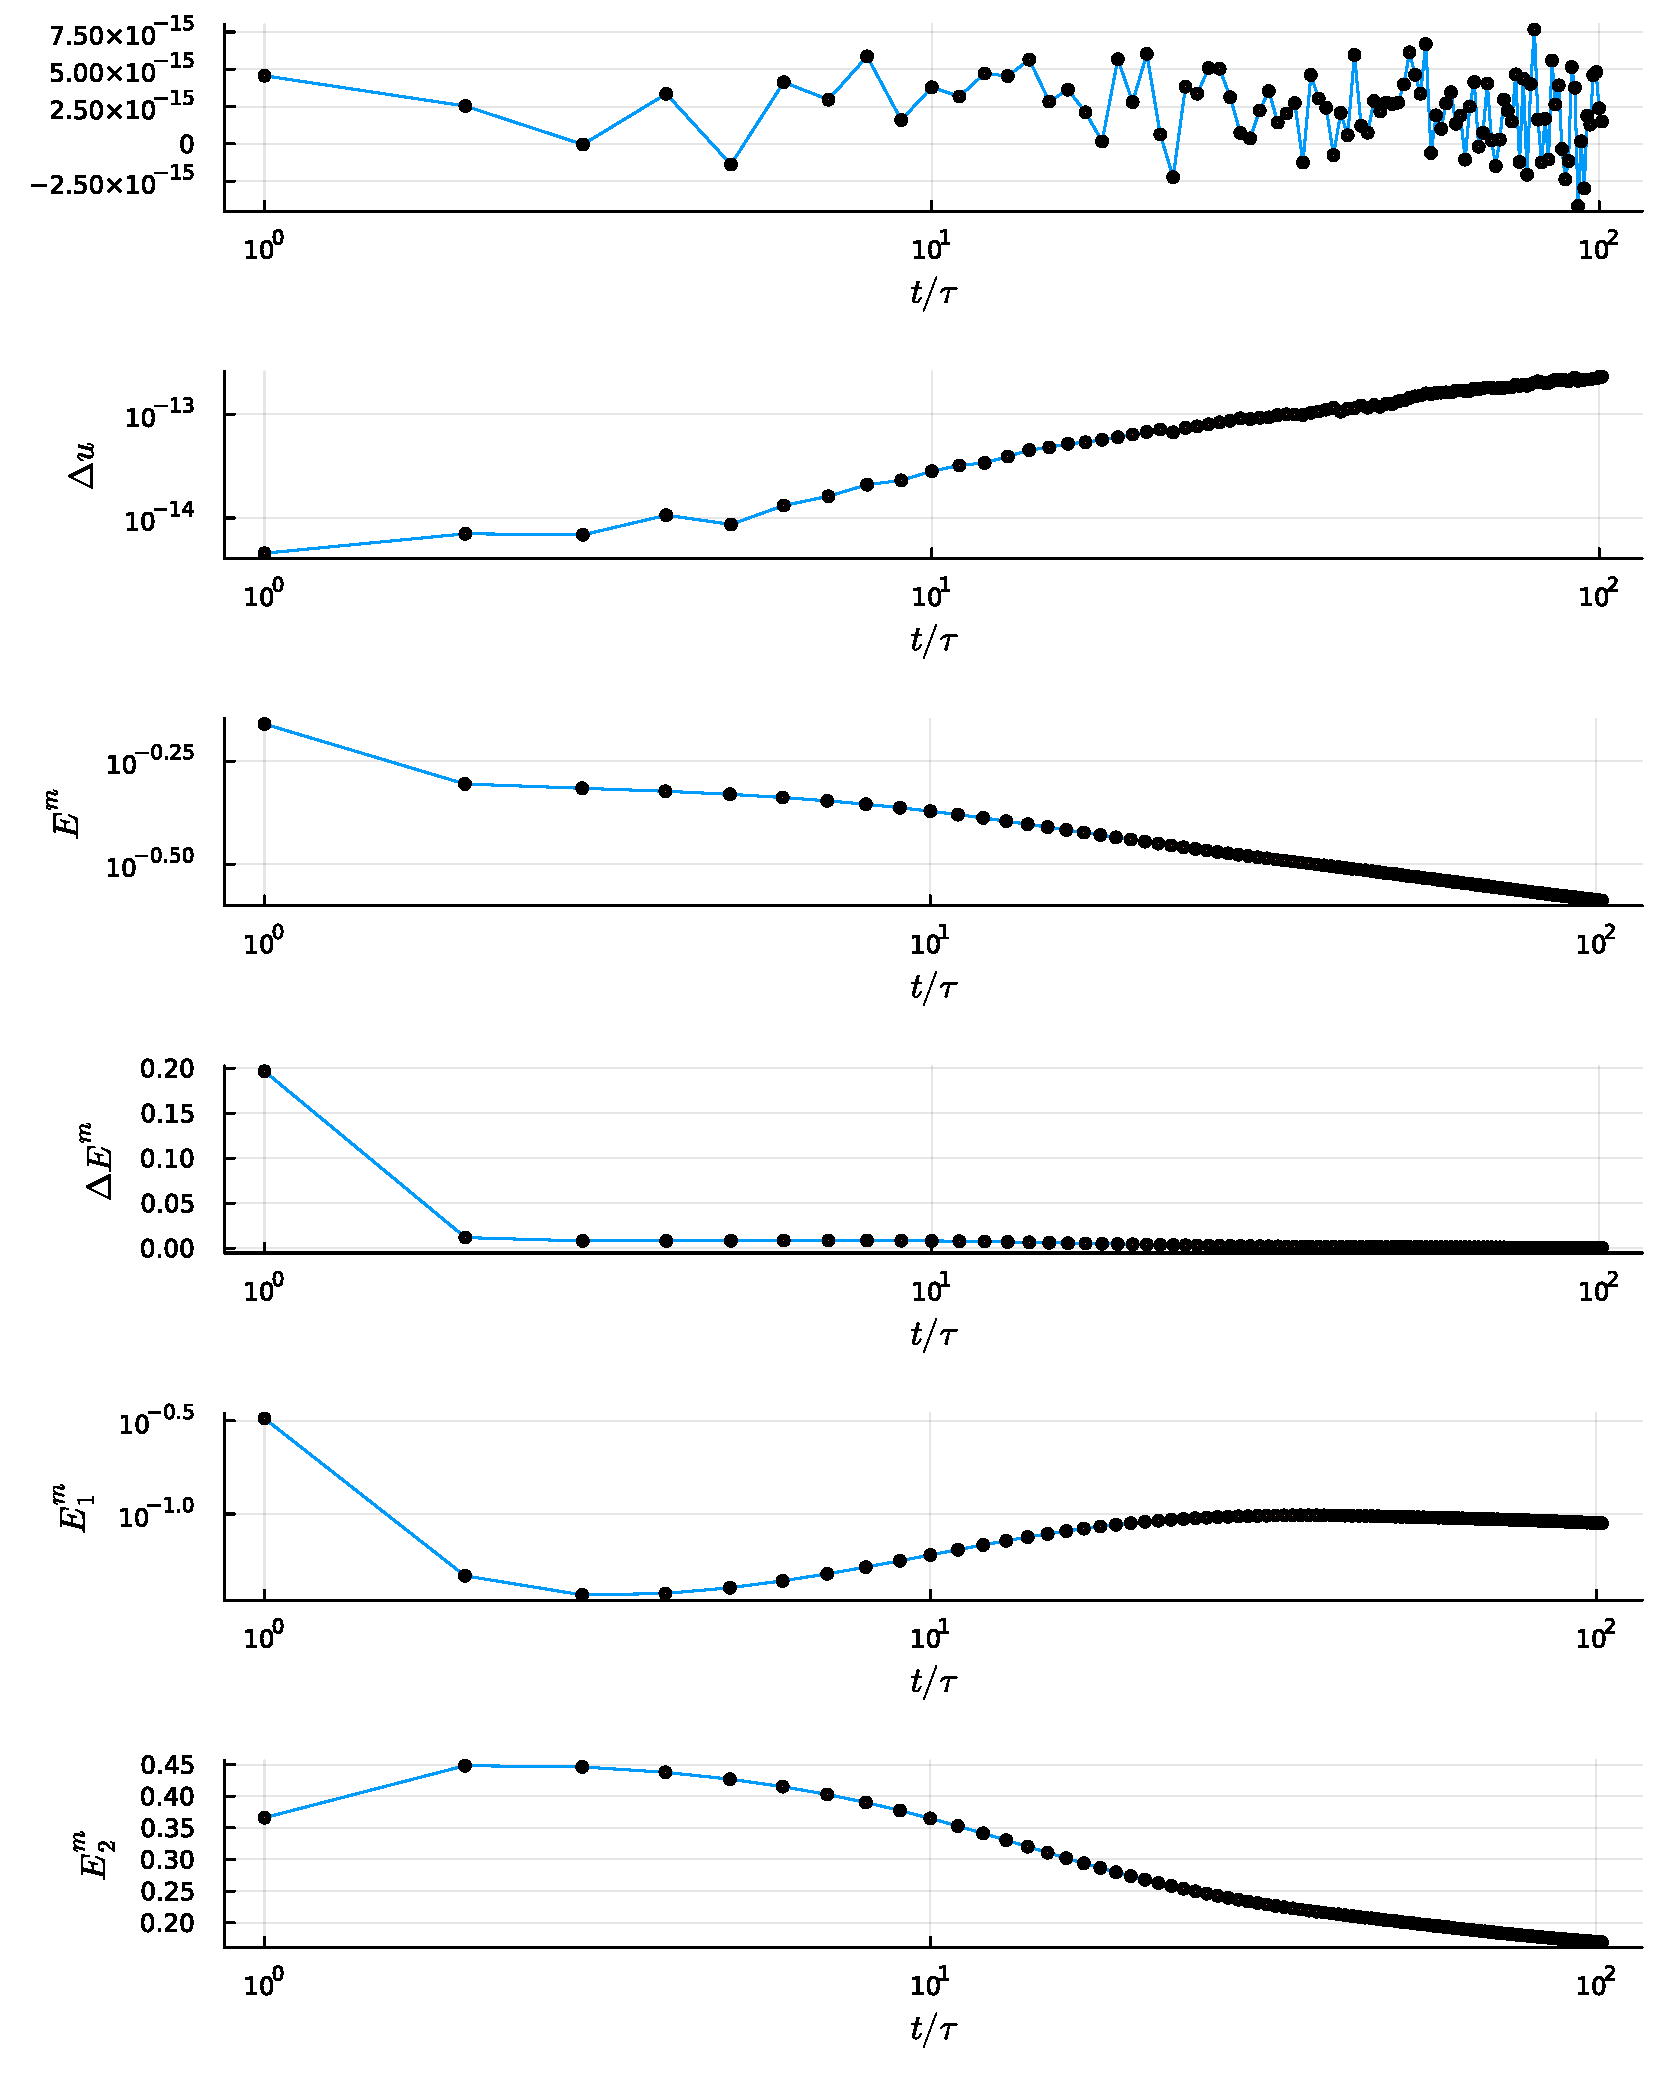
\includegraphics{results/physical_CH_plot.pdf}
    \caption{Evolution of the  global mass conservation $\Delta u^m$, and the local mass difference $\delta u^m$ total discrete energies $E^m$,$E^m_{1}$,$E^m_{2}$, with the corresponding local energy difference $\delta E^m$, on a circular domain and a flower-shaped domain. }
    \label{fig:physical_CH_plot}
\end{figure}


\begin{figure}[]
    \centering
    \hfill
    \subfloat[$m=0$]{
        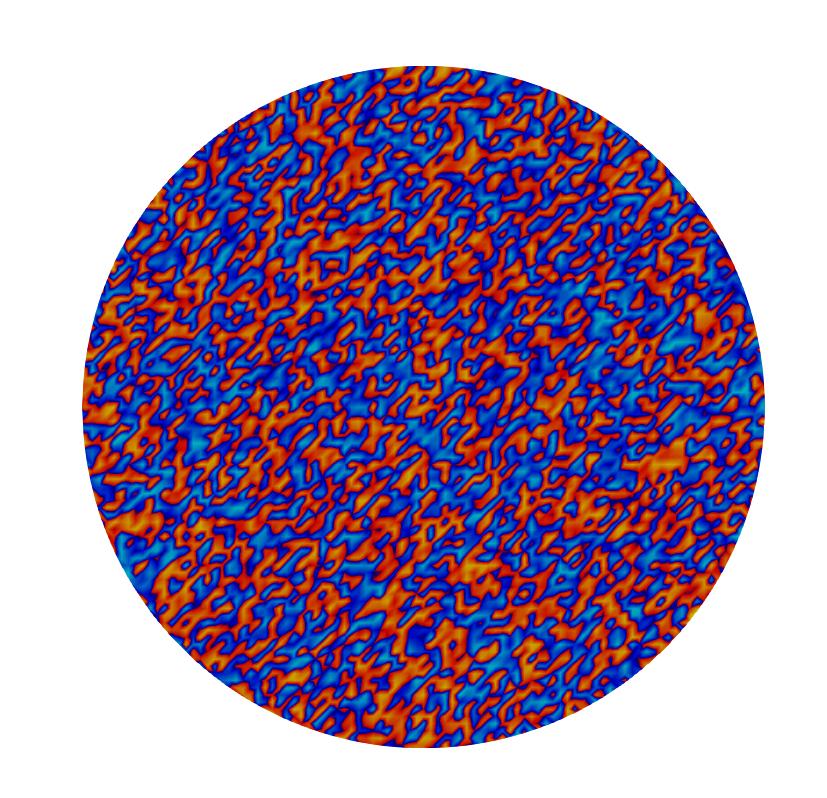
\includegraphics[width=0.3\textwidth]{results/illustration/c0.png}
    }\hfill
    \subfloat[$m=2$]{
        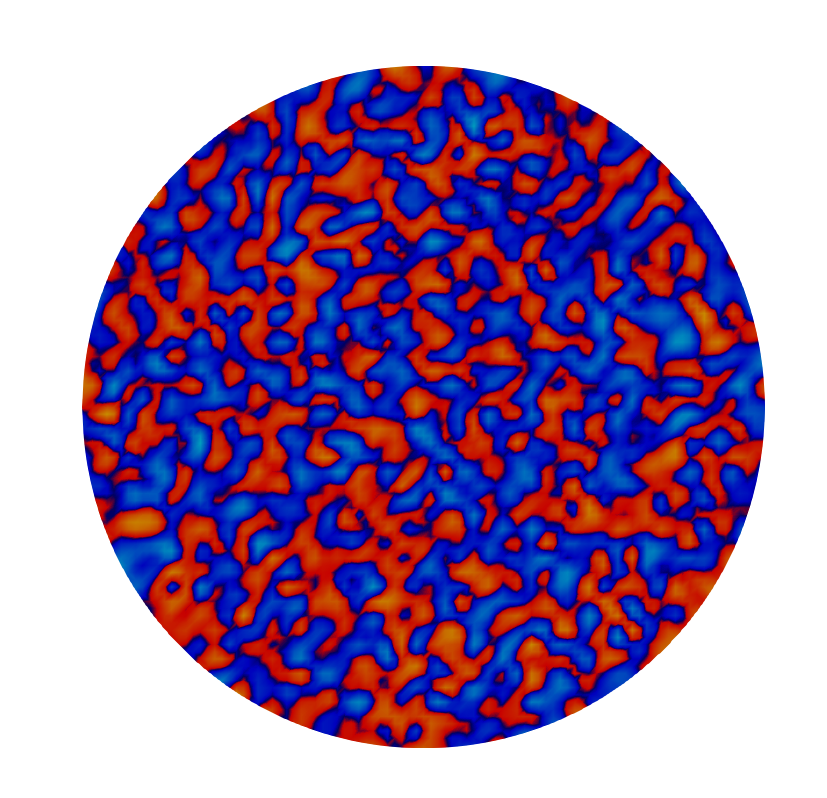
\includegraphics[width=0.3\textwidth]{results/illustration/c2.png}
    }
    \hfill
    \subfloat[$m=10$]{
        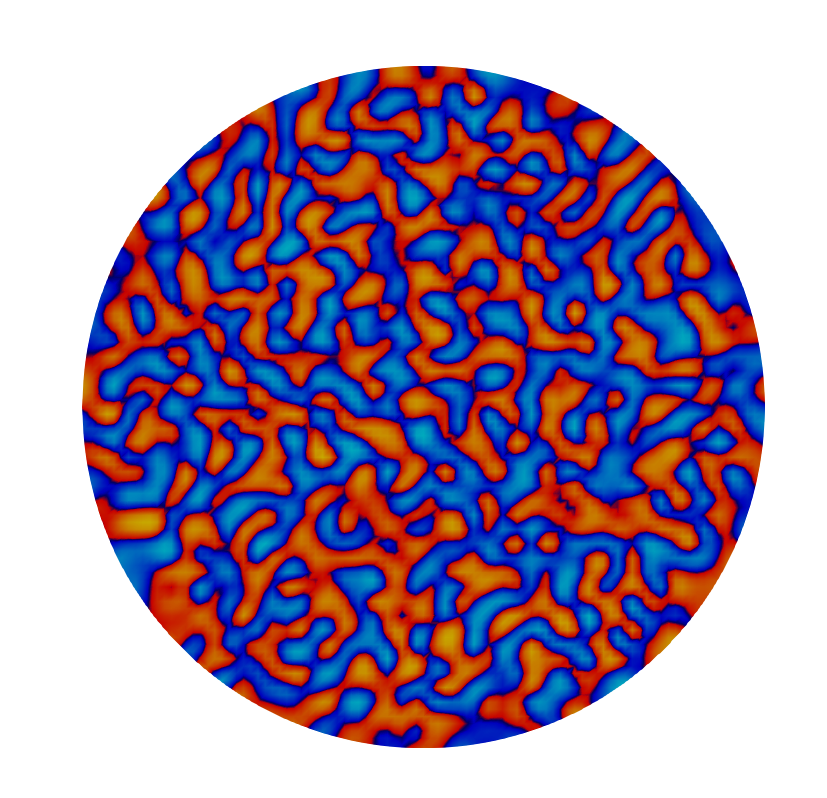
\includegraphics[width=0.3\textwidth]{results/illustration/c10.png}
    }
    \\
    \vspace{10pt}
    \hfill
    \subfloat[$m=50$]{
        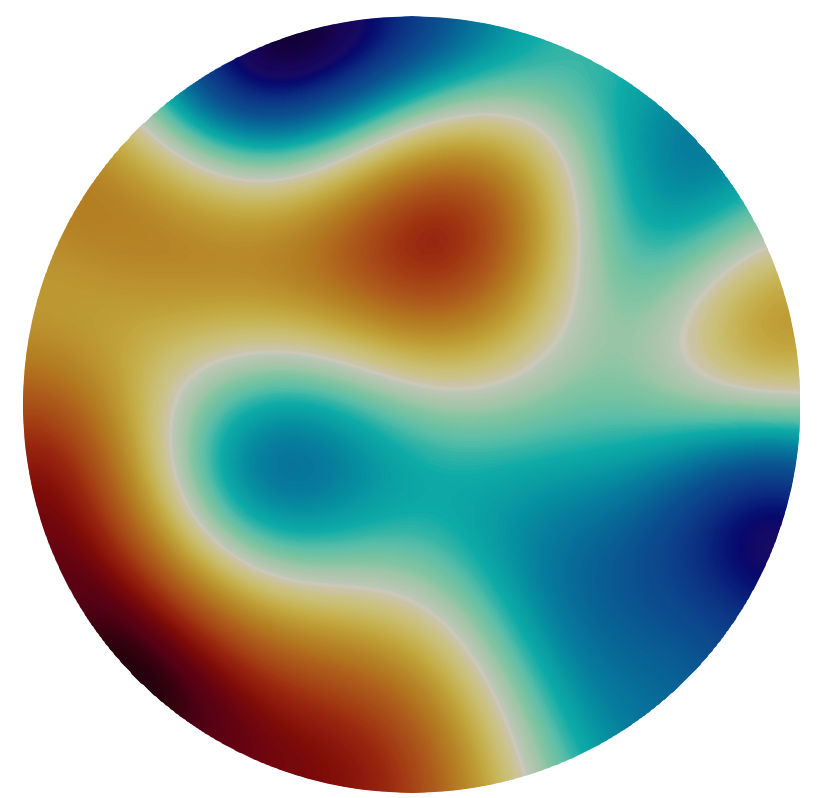
\includegraphics[width=0.3\textwidth]{results/illustration/c50.png}
    }
    \hfill
    \subfloat[$m=200$]{
        
\includegraphics[width=0.3\textwidth]{results/illustration/c200.png}
    }\hfill
    \subfloat[$m=500$]{
        
\includegraphics[width=0.3\textwidth]{results/illustration/c500.png}
    }
    \\
    \vspace{10pt}
    \hfill
    \subfloat[$m=1000$]{
        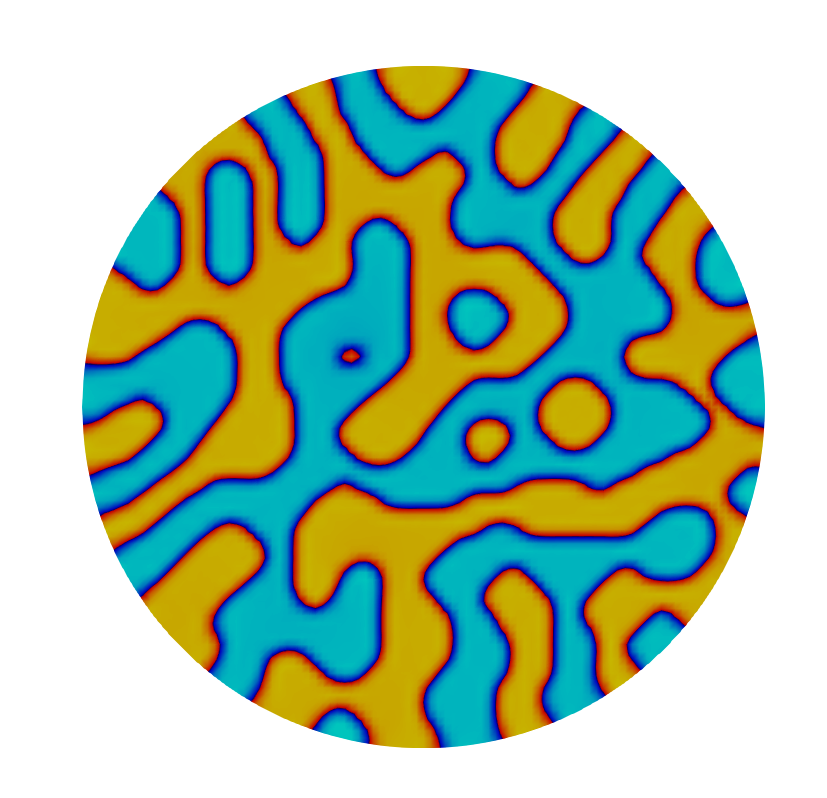
\includegraphics[width=0.3\textwidth]{results/illustration/c1000.png}
    }
    \hfill
    \subfloat[$m=5000$]{
        
\includegraphics[width=0.3\textwidth]{results/illustration/c5000.png}
    }\hfill
    \subfloat[$m=10000$]{
        
\includegraphics[width=0.3\textwidth]{results/illustration/c10000.png}
    }
    \vspace{10pt}
        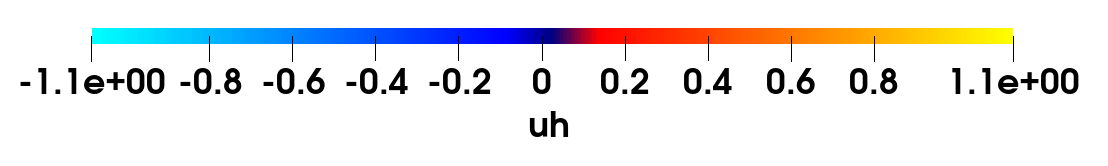
\includegraphics[width=0.8\textwidth]{results/illustration/colobar.png}

    \caption{Illustration of simulations of the Cahn-Hilliard equation on the circle domain for $t\in \left[ 0, 10000\tau  \right] $.}
        \label{sub:fig:ill_circle}
\end{figure}

\begin{figure}[]
    \centering
    \hfill
    \subfloat[$m=0$]{
        
\includegraphics[width=0.3\textwidth]{results/illustration/f0.png}
    }\hfill
    \subfloat[$m=2$]{
        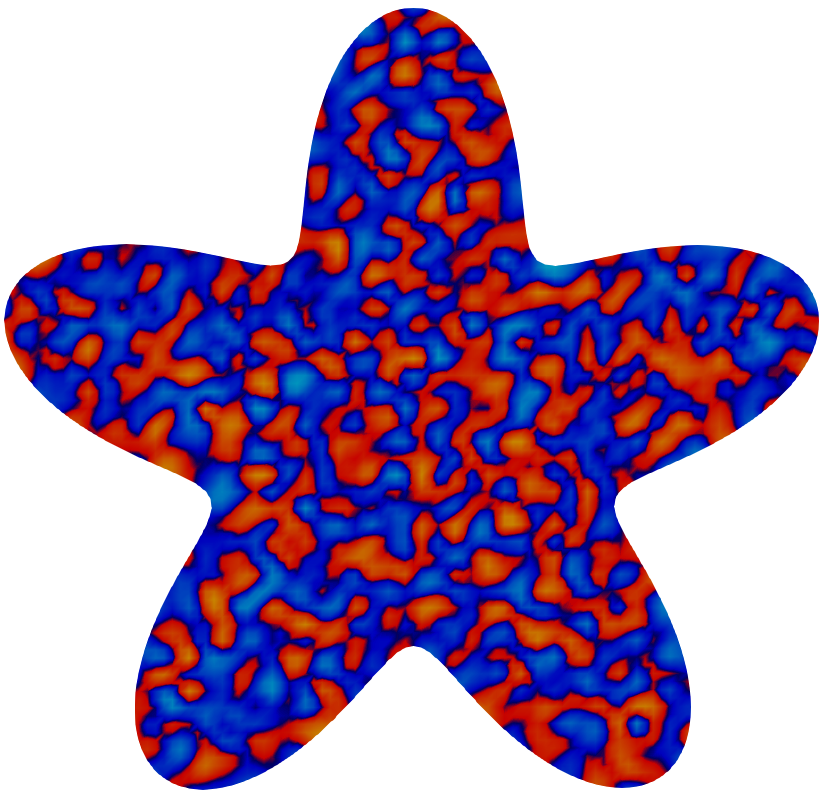
\includegraphics[width=0.3\textwidth]{results/illustration/f2.png}
    }
    \hfill
    \subfloat[$m=10$]{
        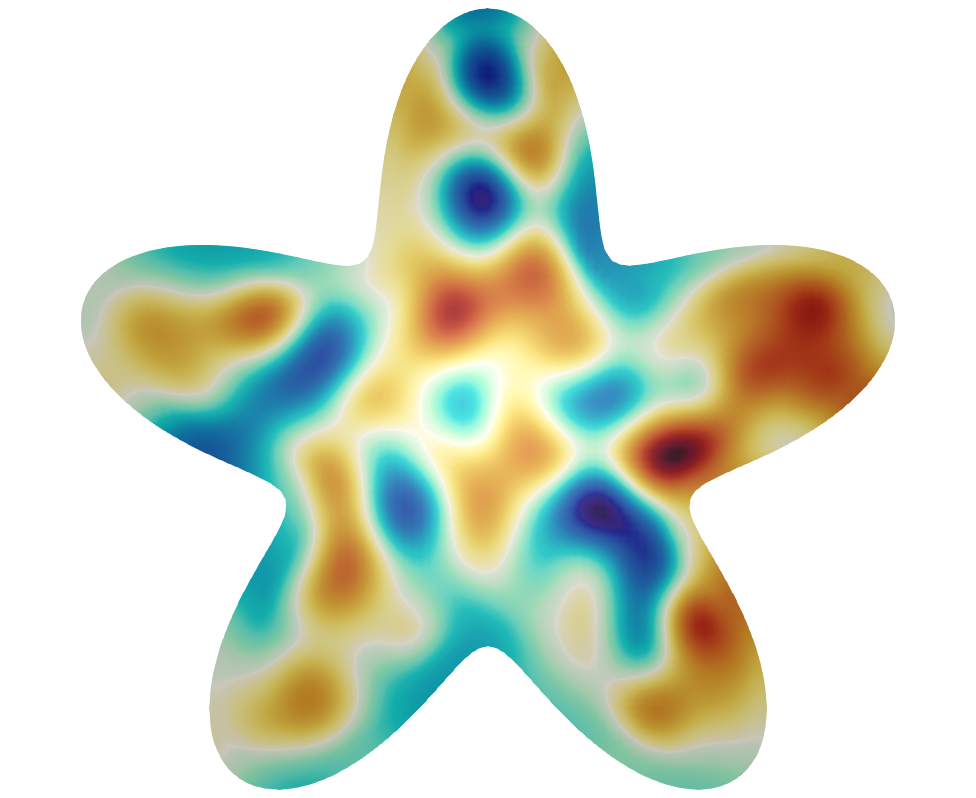
\includegraphics[width=0.3\textwidth]{results/illustration/f10.png}
    }
    \\
    \vspace{10pt}
    \hfill
    \subfloat[$m=50$]{
        
\includegraphics[width=0.3\textwidth]{results/illustration/f50.png}
    }
    \hfill
    \subfloat[$m=200$]{
        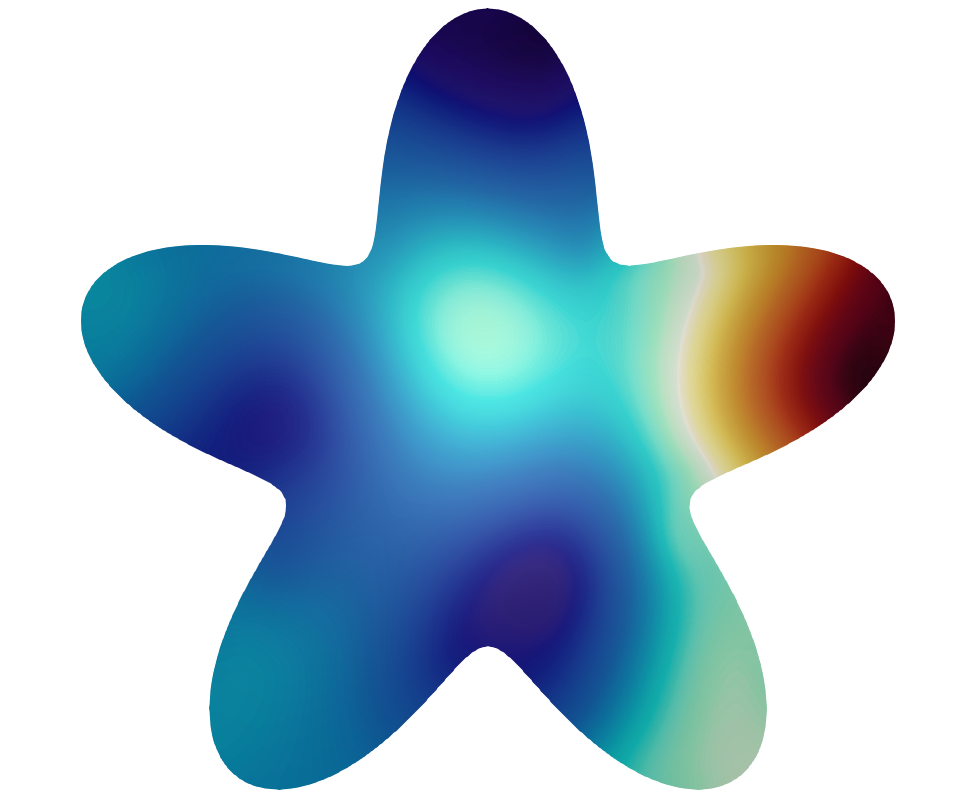
\includegraphics[width=0.3\textwidth]{results/illustration/f200.png}
    }\hfill
    \subfloat[$m=500$]{
        
\includegraphics[width=0.3\textwidth]{results/illustration/f500.png}
    }
    \\
    \vspace{10pt}
    \hfill
    \subfloat[$m=1000$]{
        
\includegraphics[width=0.3\textwidth]{results/illustration/f1000.png}
    }
    \hfill
    \subfloat[$m=5000$]{
        
\includegraphics[width=0.3\textwidth]{results/illustration/f5000.png}
    }\hfill
    \subfloat[$m=10000$]{
        
\includegraphics[width=0.3\textwidth]{results/illustration/f10000.png}
    }
    \vspace{10pt}
        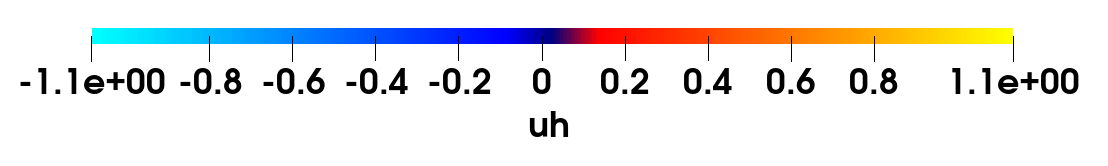
\includegraphics[width=0.8\textwidth]{results/illustration/colobar.png}
    \caption{Illustration of simulations of the Cahn-Hilliard equation on the flower domain for $t\in \left[ 0, 10000\tau  \right] $.}
        \label{sub:fig:ill_flower}
\end{figure}



In our experiments, we defined the initial function $u_{0}(x)$ as the uniform samples from the interval $[-1, 1]$ for each node. That is, for each node $a_{i}$, $u_{0}(a_{i})$ is a sample from the uniform distribution on the interval $[-1, 1]$. This
applies for all $i = 1, \ldots, N$, where $N$ is the total number of degrees of freedom in our system. The node $a_{i}$ is associated with the nodal basis for all $N$ degrees of freedom, as discussed for the discrete system
\eqref{eq:discretized_system}. We again used a square background mesh with length $L=2.7$ and mesh size $h=\frac{L}{n}$ for $n=2^{7}$. For an illustration of the active set $\mathcal{T}_{h} $ (defined in Section \ref{sub:unfitted_mesh}), see Figure \ref{sub:fig:active_mesh}.

\begin{figure}[H]
    \centering
    \hfill
    % \subfloat[]{
        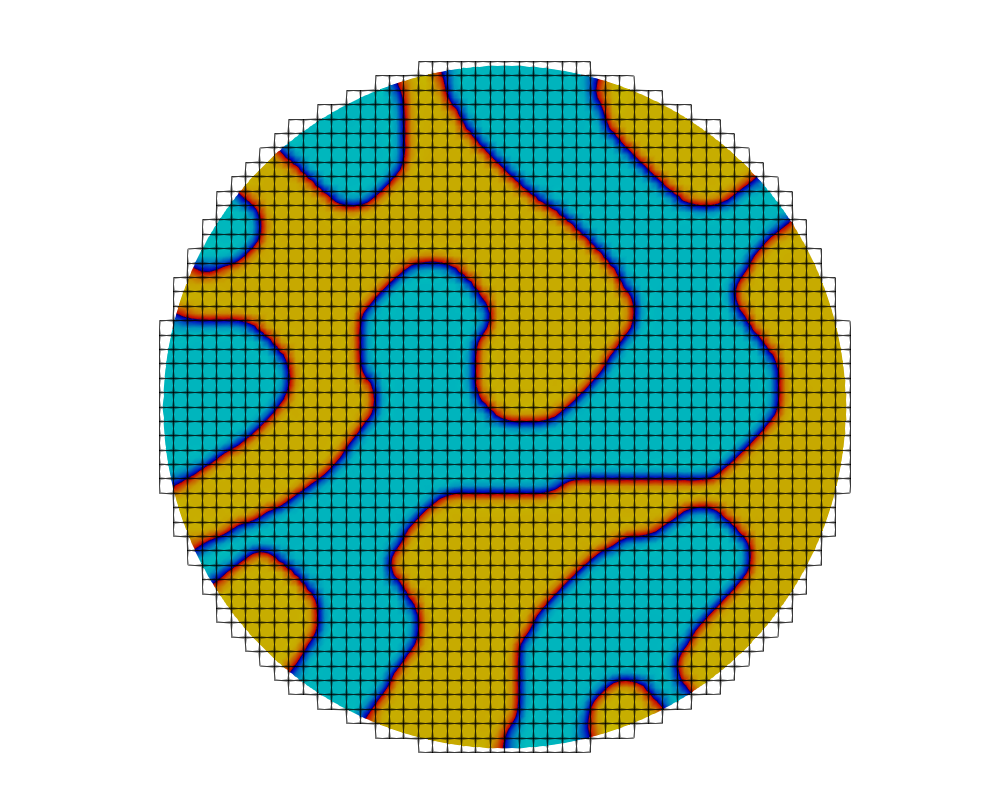
\includegraphics[width=0.45\textwidth]{results/illustration/active_circle.png}
    % }
    \hfill
    % \subfloat[]{
        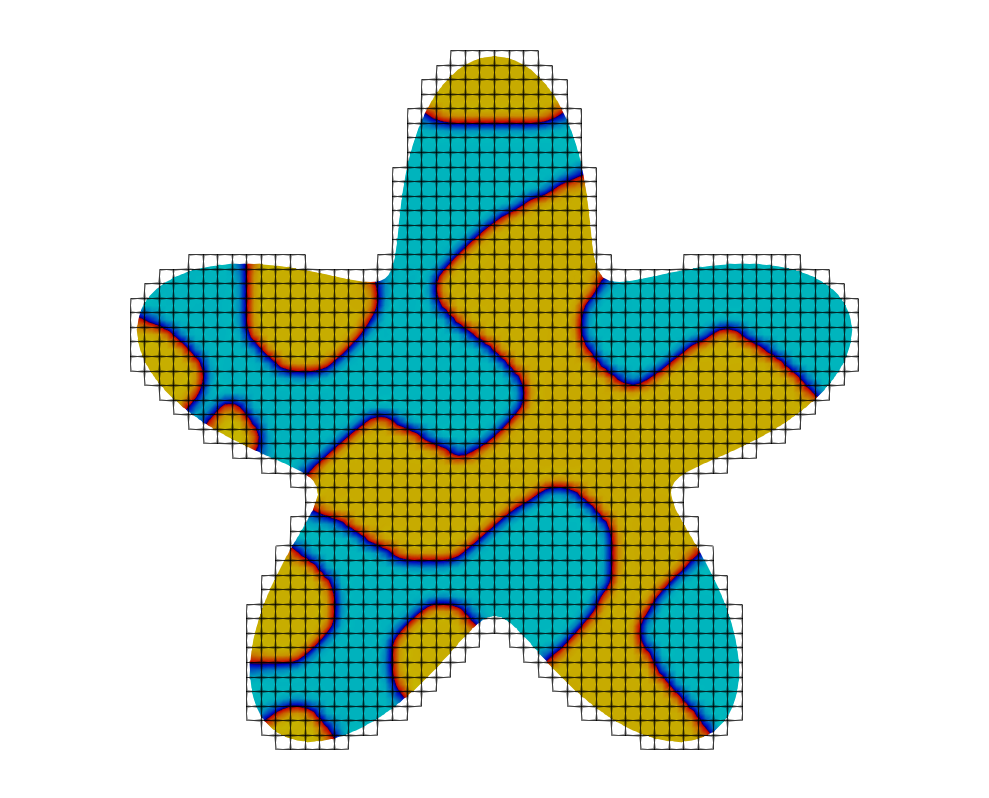
\includegraphics[width=0.45\textwidth]{results/illustration/active_flower.png}
    % }
    \caption{Illustration of the active mesh $\mathcal{T}_{h} $.}
    \label{sub:fig:active_mesh}
\end{figure}


We ran the simulation on the for the flower domain \eqref{eq:flower} and the circular domain \eqref{eq:circle}, illustrated in Figure \ref{sub:fig:ill_flower} and \ref{sub:fig:ill_circle}. The corresponding plots of the mass conservation and energy decrease are presented
in the Figure \ref{fig:physical_CH_plot}, and confirm the expected physical properties of the Cahn-Hilliard equation. The global relative error $\Delta u^{m}_{h}$ and $\delta u^{m}_{h}$ demonstrating that the mass is conserved. We also observe that the energy functional
$E(u_h)$ monotonically decreases over time and that $\delta E^{m} >0$, signifying the systems tendency to seek a state of minimal energy. Take note that $E^{m}{1}$ and $E^{m}{2}$ are interconnected in such a way that if the value of one increases, the other will correspondingly decrease to maintain balance, and vice versa.



\subsection{Note on the manufactured solution}%
\label{sub:the_problem}

While the report is not consisting of a numerical convergence analysis of the Cahn-Hilliard problem, we still present a framework for manufactured solutions for non-homogeneous boundary conditions. Let $ u( x,0) =  u_{0}$ then is Cahn-Hilliard with
non-homogeneous boundary conditions as follows,
\begin{subequations}
    \label{eq:ch_gen}
    \begin{align}
    \label{eq:ch_gen:a}
        \partial _{t} u + \Delta  \left(  \varepsilon^2  \Delta u - f( u) \right)   &= g_{0}( x)   \quad \text{ in } \Omega,  \\
        \partial _{n} u &= g_{1}( x)  \quad \text{ on } \Gamma,  \\
        \partial _{n}    \Delta u   &= g_{2}(x)  \quad \text{ on } \Gamma,
    \end{align}
\end{subequations}
where we defined $f( u) = F'( u) =u( u^2 -1)  $ for $F( u) = \frac{1}{4}( u^{2} - 1)^{2} $ and the domain $\Omega \subset \mathbb{R} ^{d} $  for $d = 2,3$. In contrast to the standard version presented in the introduction \eqref{eq:strongch}, this
version is generalized to also holds for for functions $g_{0},g_{1},g_{2}: \Omega \to\mathbb{R}   $. While the standard version may be physical correct, this version creates flexibility so we can easily construct manufactured solution on complex domains.

    Designing a manufactured solution using $g_{0}( \cdot ) $ may be temping with the formulation \eqref{eq:ch_gen:a}. However, observe that expanding the Laplacian we get,
    \begin{equation}
    \begin{split}
        \Delta  \left(  \varepsilon^2  \Delta u - f( u) \right) & = \varepsilon^2 \Delta^2 u -  \Delta f( u) \\
                                                                                    &= \varepsilon^{2} \Delta ^2 u  - 3( 2u \| \nabla u \|_{ 2 }^{ 2 } + u^{2}  \Delta u )   \\
    \end{split}
    \end{equation}
Here we applied the chain rule twice and inserted the derivatives.
\begin{equation}
    \label{eq:nonlinear_laplace}
    \begin{split}
\Delta f( u)  &= \nabla \cdot \nabla f( u)  = \nabla \cdot  \left[ f' ( u) \partial _{x_{1}}u, \ldots, f' ( u) \partial _{x_{d}}u \right] ^{T} \\
& =  f'' ( u)( ( \partial _{x_{1}}u )^{2} + \ldots +( \partial _{x_{d}}u )^{2} ) +  f' ( u)( \partial _{x_{1} x_{1}}u + \ldots +   \partial _{x_{d} x_{d}}u ) \\
&=  f'' ( u) \| \nabla u \|_{ 2 }^{ 2 } + f' ( u)  \Delta u  = 6u \| \nabla u \|_{ 2 }^{ 2 } + 3u^{2}  \Delta u
    \end{split}
\end{equation}

% Our goal is to write the Cahn Hilliard equation on weak form.
% Assume that $\Omega  \subset \mathbb{R} ^{d}$ with a $\Gamma $ in $C^2$.
%  Let $u \in  H^{4}( \Omega ) $ and $v \in V_{h} $.
% Now, expanding the first Laplace operator from a weak point of view is it clear that
% \[
%  ( \Delta ( \varepsilon  \Delta u - \frac{1}{\varepsilon } f( u) ) ,v )_{\Omega } = \varepsilon ( \Delta^{2} u ,v )_{\Omega } - \frac{1}{\varepsilon } ( \Delta f( u)  ,v )_{\Omega }.
% \]
% Hence, this makes it natural to associate the biharmonic $( \Delta ^2 u,v)_{\Omega } $ with bilinear forms $A_{h}( \cdot ,\cdot ) $ , however, in this section will we only consider the Laplace
% variant $a^{L}( \cdot ,\cdot ) $.
We now seek to find a weak form of the nonlinear term with non homogeneous boundary conditions.
\begin{lemma}[Semi-linear form]
    Let $u \in H^4( \Omega ) $ be solution to \eqref{eq:ch_gen} and $v_{h} \in V_{h}$ the test function.
Then can we rewrite the nonlinear term into the corresponding semi-linear form $c_{h}( \cdot ,\cdot )  $ for the nonlinear term $( -\Delta f( u) , v_{h})_{\Omega }$ into two consistent formulations.
\begin{align}
    \label{eq:ch:1}
      c^{1}_{h} ( u,v_{h})  & = ( f' ( u) \nabla u, \nabla v_{h} )_{\Omega }  - ( f'( u)  g_{1}   ,  v_{h})_{\Gamma } \\
    \label{eq:ch:2}
        c^{2}_{h} ( u,v_{h})  & = -( f( u), \Delta v_{h} )_{\Omega }+  ( f( u) , \jump{ \partial _{n}v_{h} }  )_{\mathcal{F} _{h}^{int}} + ( f(u), \partial _{n} v_{h})_{\Gamma  }  - ( f'( u)  g_{1}   ,  v_{h})_{\Gamma }
\end{align}
% \begin{remark}
%     Be aware that the both formulations are consistent and if we replace $u \in H^{4}( \Omega ) $ with  $u_{h} \in  V_{h}$ we have two different discrete formulations.
% \end{remark}

\end{lemma}
% \todo[inline]{ I criticize \cite[ Remark 4.1d]{feng2007fully} which says that says that finding this weak form is not possible for conforming methods (I guess $C^{0}$ is a conforming method??). }

\begin{proof}

         \textbf{Derivation of \eqref{eq:ch:1}.  }  We want to construct the first formulation. Let $T$ be an element in $\mathcal{T}_{h}$. From Greens theorem is it easy to see that
            \begin{equation}
            \label{eq:1_gr}
-(\Delta f( u) , v_{h})_{T } = (\nabla f( u), \nabla v_{h}  )_{T } - ( \partial _{n}  f( u), v_{h} )_{\partial T }
            \end{equation}
            First by utilizing that $\nabla f( u) = f' ( u) \nabla u $ and $\partial _{n}f( u)  = f' ( u)  \partial _{n}u$  and doing a summation over the triangles  is it clear that \[
            ( -\Delta f( u),v_{h} )_{\Omega  } =(f' ( u) \nabla u, \nabla v_{h}  )_{\Omega  } - (   f' ( u)\partial _{n}u, v_{h} )_{\partial \mathcal{T}_{h}  }
            \]
            Iterating over the facets is it clear that \[
                \begin{split}
            (   f' ( u)\partial _{n}u, v_{h} )_{\partial \mathcal{T}_{h}  } & = \sum_{F \in \mathcal{F}_{h}  }^{} \int_{F}^{}   \jump{ f' ( u)\partial _{n}u, v_{h} } \\
                                                                        & =  ( \jump{ f' ( u) \partial _{n}u },  \mean{v_{h}}    )_{\mathcal{F}^{int}_{h} } + ( \mean{ f' ( u) \partial _{n}u }, \jump{ v_{h} }    )_{\mathcal{F}^{int}_{h} } +  ( f' ( u)
                                                                        \partial _{n}u, v_{h}) _{\Gamma } \\
                                                                        & =  ( f' ( u) \partial _{n}u, v_{h}) _{\Gamma }
                \end{split}
            \]
            The jump terms vanishes by the regularity of $u$ and $v_{h}$. Hence, by inserting $g_{1}$ we have shown that the first formulation holds.

         \textbf{Derivation of \eqref{eq:ch:2}.  }  Applying a extra iteration of Greens theorem on \eqref{eq:1_gr} we get the following terms.
\[
    \begin{split}
-(\Delta f( u) , v_{h})_{T }  = -( f( u), \Delta v_{h} )_{T} + (f( u), \partial _{n} v_{h}  )_{\partial T} - (   f'( u)\partial _{n}u, v_{h} )_{\partial T } .
    \end{split}
\]
Now, by doing a summation of all triangles it is clear that this holds.
\begin{equation}
\label{eq:f_g2}
-(\Delta f( u) , v_{h})_{\Omega  }  = -( f( u), \Delta v_{h} )_{\Omega } + (f( u), \partial _{n} v_{h}  )_{\partial \mathcal{T}_{h} } - (   f'( u)\partial _{n}u, v_{h} )_{\partial \mathcal{T}_{h}  }
\end{equation}
It comes evident from the first step of the proof that $ (   f'( u)\partial _{n}u, v_{h} )_{\partial \mathcal{T}_{h}  } = (   f'( u)\partial _{n}u, v_{h} )_{\Gamma }$, hence, we only need to compute the term $(f( u), \partial _{n} v_{h}  )_{\partial
\mathcal{T}_{h} }$ on the facets. \[
    \begin{split}
(f( u), \partial _{n} v_{h}  )_{\partial
\mathcal{T}_{h} } & = \sum_{F\in \mathcal{F} _{h}}^{} \int_{F}^{}\jump{ f( u), \partial _{n} v_{h}  } \\
& =  (\jump{ f( u)  }  , \mean{ \partial _{n} v_{h} }    )_{ \mathcal{F}_{h}^{int} } +(\mean{ f( u)  }  , \jump{ \partial _{n} v_{h} }    )_{ \mathcal{F}_{h}^{int} } + (f( u), \partial _{n} v_{h}  )_{\Gamma } \\
&=  (\mean{ f( u)  }  , \jump{ \partial _{n} v_{h} }    )_{ \mathcal{F}_{h}^{int} } + (f( u), \partial _{n} v_{h}  )_{\Gamma }
    \end{split}
\]
Again one of the jump terms vanishes because of the regularity of $u$.
Inserting the result into \eqref{eq:f_g2} have we shown that the second formulation also holds.
\end{proof}


Combining the full general Cahn-Hilliard problem in \eqref{eq:ch_gen} with the semi-linear forms\eqref{eq:ch:1} and the CutCIP biharmonic problem \eqref{eq:discrete_CutCIP_prob}, we get the following scheme.
\begin{equation}
    ( \partial _{t}u_{h}, v_{h})_\Omega + \varepsilon^2  A_{h}( u_{h},v_{h}) + c_{h}( u_{h},v_{h})   =   l_{h}(v_{h}) \quad  \forall u_{h}, v_{h} \in V_{h}
\end{equation}

To illustrate, assume we use the Laplace formulation presented in \eqref{eq:laplace_prob} integrated into \eqref{eq:discrete_CutCIP_prob}, i.e. $A_{h}( u_{h}, v_{h}) = a^{L}_{h}( u_{h}, v_{h}) + g_{h}( u_{h}, v_{h})   = l_{h}^{L}( v_{h})$. Due to the $\varepsilon $ scaling, we ultimately
arrive at the following modification.
 \begin{equation}
    l_{h}^{L}( v_{h})  =  \left( g_{0}, v_{h} \right) _{\Omega } -  \varepsilon^2 ( g_{2},  v_{h} )_{\Gamma }  -  \varepsilon^2 ( g_{1}, \Delta  v_{h}  )_{\Gamma }  + \varepsilon^2 \frac{\gamma }{h} ( g_{1}, \partial _{n} v_{h}  )_{\Gamma }
 \end{equation}
 Hence, we arrived at a system which can easily be used to construct manufactured solution.


    % \newpage
% \section{Appendix}%
% \label{sec:appendix}

% \subsection{The Space $L^{2} \left( \Omega  \right)$ }%
% \label{sub:l_2_space}

% Using the definition from \cite{manzoni2021optimal} and we let $\Omega $ be a an open set in $\mathbb{R} ^{d}$ and $p \in \mathbb{R} $  such that $p \ge 1$. Then we denote
% $L^{p}\left( \Omega  \right) $ to be the set of measurable function $u: \Omega \to \mathbb{R} $ such that  it is equipped
% in a finite Banach space \[
% \|u\|_{L^{p}\left( \Omega  \right)}^{} = \left( \int_{\Omega }^{} \left\lvert u \right\rvert ^{p}
% \right)^{\frac{1}{p}}.
% \]

% Now let $u,v: \Omega  \to \mathbb{R} $. Then is $L^{2}\left( \Omega  \right)$ a Hilbert space when the inner product is
% finite such that this exists \[
% \left( u,v \right)_{L^{p}\left( \Omega   \right)} = \int_{\Omega }^{} uv  .
% \]
% If the integral is finite do we say that $u,v \in L^{p}\left( \Omega  \right)$.



% \subsection{The Space $H^{m} \left( \Omega  \right)$, $m>1$  }%
% \label{sub:h_2_space}

% Again using the definition from \cite{manzoni2021optimal}. Let $\alpha=\left( \alpha _{1}, \ldots, \alpha _{d} \right),
% \quad \alpha \ge  0$, such that $\left\lvert \alpha  \right\rvert = \sum_{i=1}^{d} \alpha _{i} $. Now we define
% the space \[
% H^{m}\left( \Omega  \right) = \left\{ u \in L^2\left( \Omega  \right) : D^{\alpha } u \in L^2\left( \Omega  \right)\quad
% \forall \alpha : \left\lvert \alpha  \right\rvert  \le  m \right\}.
% \]


% Suppose that $u,v$ is measurable functions. We can now define $u \in H^{m}\left( \Omega  \right)$  the Banach space is
% finite . \[
% \|u\|_{H^{m}\left( \Omega  \right)}^{} = \left( \|u\|_{L^2\left( \Omega  \right)}^{}  + \sum_{k=1}^{m}
% \left\lvert u \right\rvert ^2 _{H^{k}\left( \Omega  \right)} \right), \quad \left\lvert u \right\rvert_ { H^{k} \left(
% \Omega  \right) }  = \sqrt{\sum_{\left\lvert \alpha  \right\rvert = k  }^{} \| D^{\alpha }u \|_{L^2\left( \Omega  \right)
% }^{ 2 } }
%  \]

%  Similarly for the finite Hilbert space \[
%  \left( u,v \right)_{ H^{m} \left( \Omega  \right)}  = \sum_{\left\lvert \alpha  \right\rvert  \le  m}^{}  \int_{\Omega }^{}
%  D^{\alpha } u D^{\alpha } v
%  \]









    \newpage
    \printbibliography

\end{document}
